% =====================================================================
%  CENG 252 -- Study Notes, Lectures 6--10
%  Nonelementary kinetics (PSSH, chain reactions, enzymes) and
%  heterogeneous catalysis (Langmuir--Hinshelwood, deactivation)
%  Compile with: pdflatex (run twice for the table of contents)
% =====================================================================
\documentclass[11pt]{article}
\usepackage[margin=2cm,headheight=14pt]{geometry}
\usepackage{amsmath,amssymb}
\usepackage[version=4]{mhchem}
\usepackage{tikz}
\usetikzlibrary{arrows.meta,positioning,decorations.pathmorphing,decorations.markings,calc,shapes.geometric,patterns}
\usepackage{pgfplots}
\pgfplotsset{compat=1.17}
\usepackage[most]{tcolorbox}
\usepackage{booktabs,array,tabularx,multirow}
\usepackage{enumitem}
\usepackage{fancyhdr}
\usepackage{xcolor}
\usepackage{lmodern}
\usepackage[T1]{fontenc}
\usepackage{microtype}
\usepackage{multicol}
\usepackage[colorlinks=true,linkcolor=blue!50!black,urlcolor=blue!50!black]{hyperref}

\setlist{itemsep=2pt,topsep=3pt}
\setlength{\parindent}{0pt}
\setlength{\parskip}{4pt}

\pagestyle{fancy}
\fancyhf{}
\lhead{\small CENG 252 \textbullet\ Study Notes, Lectures 6--10}
\rhead{\small \nouppercase{\leftmark}}
\cfoot{\small \thepage}

% ---------- colours and boxes ----------
\definecolor{keyblue}{RGB}{0,84,147}
\definecolor{warnred}{RGB}{176,30,30}
\definecolor{tipgreen}{RGB}{20,110,60}
\definecolor{stepgray}{RGB}{90,90,90}

\newtcolorbox{keyresult}[1][Key result]{enhanced,breakable,colback=keyblue!5,colframe=keyblue,
  fonttitle=\bfseries,title={#1},left=4pt,right=4pt,top=2pt,bottom=2pt}
\newtcolorbox{mistake}[1][Common mistake]{enhanced,breakable,colback=warnred!5,colframe=warnred,
  fonttitle=\bfseries,title={#1},left=4pt,right=4pt,top=2pt,bottom=2pt}
\newtcolorbox{examtip}[1][Exam tip]{enhanced,breakable,colback=tipgreen!5,colframe=tipgreen,
  fonttitle=\bfseries,title={#1},left=4pt,right=4pt,top=2pt,bottom=2pt}
\newtcolorbox{summarybox}[1][]{enhanced,breakable,colback=white,colframe=black!60,
  fonttitle=\bfseries,title={#1},left=4pt,right=4pt,top=2pt,bottom=2pt}

\newcommand{\step}[1]{\par\smallskip\textcolor{stepgray}{\textbf{Step #1.}}\ }
\newcommand{\fogler}[1]{\hfill{\small\textit{\textcolor{keyblue}{Fogler: #1}}}}
% adsorbed species, e.g. \AS{A} -> A.S
\newcommand{\AS}[1]{\mathrm{#1\!\cdot\!S}}
\newcommand{\Cv}{C_{v}}
\newcommand{\Ct}{C_{t}}
\newcommand{\rxn}[1]{\xrightarrow{\;#1\;}}
\newcommand{\eqm}{\rightleftharpoons}

\begin{document}

% ===================== TITLE =====================
\begin{center}
{\LARGE\bfseries CENG 252: Chemical Reaction Engineering}\\[4pt]
{\Large Study Notes for Lectures 6--10}\\[4pt]
{\large Nonelementary Kinetics \textbullet\ Enzymes \textbullet\ Catalysis \textbullet\ Catalyst Deactivation}\\[6pt]
{\small Based on the lecture slides (Z.~Chen) and Fogler, \emph{Elements of Chemical Reaction Engineering}
(3rd ed.\ Ch.~7; 4th/5th ed.\ Ch.~10)}
\end{center}

\begin{summarybox}[How to use these notes]
\begin{itemize}
\item Each section starts with the \textbf{idea in one sentence}, then the \textbf{derivation} written out step by step
(no skipped algebra), then a \textbf{boxed key result}.
\item \textcolor{warnred}{\textbf{Red boxes}} are common mistakes, plus a few typos on the lecture slides.
Read them: they are where exam points are lost.
\item \textcolor{tipgreen}{\textbf{Green boxes}} are exam tips: which shortcut to use, and what the grader looks for.
\item The last section is a \textbf{2-page formula summary}. The exam is closed-book with a formula sheet provided, but you
must know \emph{which} equation to use and how to set it up. Practise the derivations, not memorisation.
\end{itemize}
\end{summarybox}

\tableofcontents
\newpage

% =====================================================================
\section{The Big Picture: One Method for Every Mechanism}
% =====================================================================
Lectures 6--9 all answer the same question:
\begin{center}
\emph{Given a proposed mechanism of elementary steps, what rate law does it predict, and does that rate law match experiment?}
\end{center}
The method is always the same, whether the intermediate is a free radical (Lec.~6--7), an enzyme--substrate complex
(Lec.~7), or a species adsorbed on a catalyst surface (Lec.~8--9):

\begin{center}
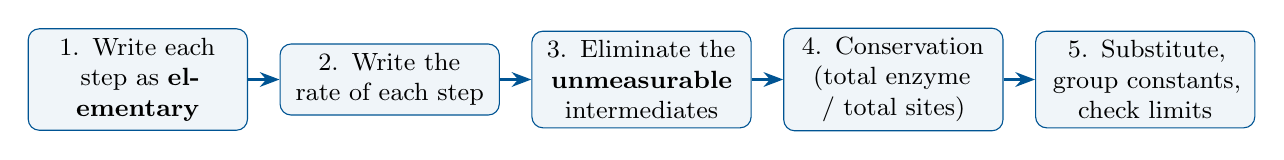
\begin{tikzpicture}[node distance=4mm and 4mm,
  box/.style={draw=keyblue,fill=keyblue!6,rounded corners,minimum height=9mm,text width=2.55cm,align=center,font=\small},
  arr/.style={-{Stealth[length=2.5mm]},thick,keyblue}]
\node[box] (a) {1. Write each step as \textbf{elementary}};
\node[box,right=of a] (b) {2. Write the rate of each step};
\node[box,right=of b] (c) {3. Eliminate the \textbf{unmeasurable} intermediates};
\node[box,right=of c] (d) {4. Conservation (total enzyme / total sites)};
\node[box,right=of d] (e) {5. Substitute, group constants, check limits};
\draw[arr] (a)--(b); \draw[arr] (b)--(c); \draw[arr] (c)--(d); \draw[arr] (d)--(e);
\end{tikzpicture}
\end{center}

\begin{center}
\renewcommand{\arraystretch}{1.25}
\begin{tabularx}{\textwidth}{>{\bfseries}l X X X}
\toprule
 & Free radicals / active intermediates & Enzymes & Heterogeneous catalysis \\
\midrule
Intermediate & $A^*$, H$\bullet$, Br$\bullet$, NO$_3^*$ & E$\cdot$S, E$\cdot$I, I$\cdot$E$\cdot$S & $\AS{A}$, $\AS{B}$, \ldots \\
How we eliminate it & PSSH: net rate of formation $=0$ & PSSH on E$\cdot$S (or equilibrium of fast steps) & Non-limiting steps are at \textbf{equilibrium} ($r/k\approx 0$) \\
Conservation law & none needed & $C_{E,t}=C_E+C_{E\cdot S}+\ldots$ & $C_t=C_v+\sum C_{i\cdot S}$ (site balance) \\
Typical result & $\dfrac{kC_A^2}{1+k'C_A}$ & $\dfrac{V_{\max}C_S}{K_M+C_S}$ & $\dfrac{kP_A}{1+K_AP_A+K_BP_B}$ \\
\bottomrule
\end{tabularx}
\end{center}

\begin{keyresult}[Reading a rate law: rules of thumb (Fogler Ch.~7 and Ch.~10)]
\begin{enumerate}
\item A species in the \textbf{denominator} collides with (or is adsorbed next to) the intermediate.
\item A \textbf{constant ``1''} in the denominator means one step is a spontaneous decomposition of the intermediate
(homogeneous kinetics), or stands for the vacant sites (catalysis).
\item A \textbf{fractional order} ($\tfrac12$, $\tfrac32$) points to a molecule splitting into two radicals or atoms
(chain initiation, or dissociative adsorption).
\item A \textbf{squared denominator} $(1+\ldots)^2$ means a dual-site surface reaction (two sites are needed).
\item A species in the \textbf{numerator but not the denominator} reacts from the gas phase (Eley--Rideal) or is not adsorbed.
\end{enumerate}
\end{keyresult}

% =====================================================================
\section{Lecture 6: Active Intermediates and the PSSH}
% =====================================================================
\fogler{3rd ed.\ \S7.1}

\subsection{What is an active intermediate?}
An \textbf{active intermediate} $A^*$ is an unstable, high-energy molecule (a free radical, an excited molecule,
an ion\ldots). It is destroyed almost as fast as it is formed, so its concentration stays \textbf{very small} and
\textbf{cannot be measured}. On the energy diagram it sits in a shallow \textbf{trough} between two barriers.

\begin{center}
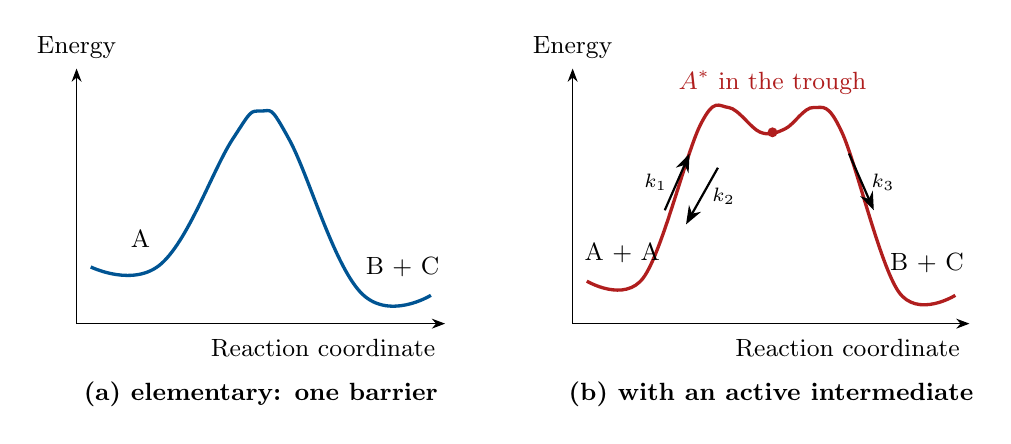
\begin{tikzpicture}[scale=0.9]
% (a) single barrier
\begin{scope}
\draw[-{Stealth}] (0,0)--(0,3.6) node[above]{\small Energy};
\draw[-{Stealth}] (0,0)--(5.2,0) node[below left,yshift=-2pt]{\small Reaction coordinate};
\draw[very thick,keyblue] plot[smooth,tension=0.7] coordinates{(0.2,0.8)(1.2,0.85)(2.2,2.6)(2.6,3.0)(3.0,2.6)(4.0,0.45)(5.0,0.4)};
\node[font=\small] at (0.9,1.2) {A};
\node[font=\small] at (4.6,0.8) {B + C};
\node[font=\small\bfseries] at (2.6,-1.0) {(a) elementary: one barrier};
\end{scope}
% (b) two barriers with trough
\begin{scope}[xshift=7cm]
\draw[-{Stealth}] (0,0)--(0,3.6) node[above]{\small Energy};
\draw[-{Stealth}] (0,0)--(5.6,0) node[below left,yshift=-2pt]{\small Reaction coordinate};
\draw[very thick,warnred] plot[smooth,tension=0.6] coordinates{(0.2,0.6)(1.0,0.65)(1.8,2.8)(2.2,3.05)(2.65,2.7)(3.0,2.75)(3.4,3.05)(3.8,2.7)(4.6,0.45)(5.4,0.4)};
\node[font=\small] at (0.7,1.0) {A + A};
\node[font=\small] at (5.0,0.85) {B + C};
\fill[warnred] (2.82,2.70) circle(2pt);
\node[font=\small,warnred,above] at (2.82,3.1) {$A^*$ in the trough};
\draw[-{Stealth},thick] (1.3,1.6) -- node[left,font=\scriptsize]{$k_1$} (1.65,2.4);
\draw[-{Stealth},thick] (2.05,2.2) -- node[right,font=\scriptsize]{$k_2$} (1.6,1.4);
\draw[-{Stealth},thick] (3.9,2.4) -- node[right,font=\scriptsize]{$k_3$} (4.25,1.6);
\node[font=\small\bfseries] at (2.8,-1.0) {(b) with an active intermediate};
\end{scope}
\end{tikzpicture}
\end{center}

\subsection{The Pseudo-Steady-State Hypothesis (PSSH)}
\begin{keyresult}[PSSH]
The \textbf{net} rate of formation of every active intermediate is zero:
\[
r_{A^*} \;=\; \sum_{i=1}^{N} r_{iA^*} \;=\; 0 .
\]
Physical meaning: $A^*$ is formed and consumed at (almost) the same rate, so its tiny concentration changes very little
compared with the reactants. PSSH lets you \textbf{solve algebraically for $C_{A^*}$} and remove it from the rate law.
\end{keyresult}

\subsection{Relative rates within one step (the most common source of error)}
For an elementary step $aA+bB\to cC$: $\dfrac{r_A}{-a}=\dfrac{r_B}{-b}=\dfrac{r_C}{c}$.
The rate constant is always defined \emph{with respect to one species}. When you write the PSSH balance for the
intermediate, convert every step's rate to the intermediate:
\begin{itemize}
\item \ce{Br2 ->[k_1] 2Br$\bullet$}, with $k_1$ defined w.r.t.\ Br$_2$: $\;-r_{1,\mathrm{Br_2}}=k_1C_{\mathrm{Br_2}}$, so
$r_{1,\mathrm{Br}\bullet}=+2k_1C_{\mathrm{Br_2}}$ \quad(factor 2).
\item \ce{NO3^* + NO ->[k_3] 2NO2}, with $k_3$ defined w.r.t.\ NO$_2$: $r_{3,\mathrm{NO_2}}=k_3C_{\mathrm{NO_3^*}}C_{\mathrm{NO}}$,
so $r_{3,\mathrm{NO_3^*}}=-\tfrac12 k_3C_{\mathrm{NO_3^*}}C_{\mathrm{NO}}$ \quad(factor $\tfrac12$).
\end{itemize}
\begin{mistake}
Forgetting the stoichiometric factor (2 or $\tfrac12$) when a step makes or uses \emph{two} of a species. Always write
which species $k_i$ refers to before you write the rate.
\end{mistake}

\subsection{Example 1: Lindemann mechanism, $-r_A=\dfrac{kC_A^2}{1+k'C_A}$}
\textbf{Experiment:} the gas-phase decomposition \ce{A -> B + C} follows $-r_A=\dfrac{kC_A^2}{1+k'C_A}$.
\textbf{Task:} propose a mechanism.

\textbf{Reading the rate law:} $C_A$ is in the denominator, so A collides with the intermediate. The ``1'' in the
denominator means $A^*$ also decomposes on its own. The $C_A^2$ in the numerator means $A^*$ is made by an A--A collision.

\textbf{Mechanism:}
\[
\text{(1)}\;\; A+A\rxn{k_1}A^*+A \qquad
\text{(2)}\;\; A^*+A\rxn{k_2}A+A \qquad
\text{(3)}\;\; A^*\rxn{k_3}B+C
\]
Step (1) activates A by collision. Step (2) deactivates $A^*$ by collision. Step (3) decomposes $A^*$ into products.
All three $k$'s are defined with respect to $A^*$.

\step{1}\textbf{Rate laws of each step, written for $A^*$} (each step is elementary, so its rate law follows from its stoichiometry):
\[
r_{1A^*}=k_1C_A^2,\qquad r_{2A^*}=-k_2C_AC_{A^*},\qquad r_{3A^*}=-k_3C_{A^*}.
\]
\step{2}\textbf{Rate of formation of product.} B is formed only in step (3), so
\[
r_B=r_{3B}=-r_{3A^*}=k_3C_{A^*}. \tag{a}
\]
This contains $C_{A^*}$, which cannot be measured, so we must eliminate it.

\step{3}\textbf{PSSH on $A^*$:}
\[
r_{A^*}=r_{1A^*}+r_{2A^*}+r_{3A^*}=k_1C_A^2-k_2C_AC_{A^*}-k_3C_{A^*}=0 .
\]
\step{4}\textbf{Solve for $C_{A^*}$.} Collect the $C_{A^*}$ terms: $k_1C_A^2=C_{A^*}(k_3+k_2C_A)$, so
\[
C_{A^*}=\frac{k_1C_A^2}{k_3+k_2C_A}. \tag{b}
\]
\step{5}\textbf{Substitute (b) into (a)}, then use \ce{A -> B + C} ($-r_A=r_B$):
\[
-r_A=r_B=\frac{k_1k_3C_A^2}{k_3+k_2C_A}.
\]
\step{6}\textbf{Match the experimental form.} Divide the numerator and denominator by $k_3$:
\[
-r_A=\frac{k_1C_A^2}{1+(k_2/k_3)C_A}=\frac{kC_A^2}{1+k'C_A},\qquad k=k_1,\quad k'=\frac{k_2}{k_3}. \;\checkmark
\]

\textbf{Limiting cases (a favourite exam question):}
\begin{itemize}
\item \textbf{High $C_A$} ($k_2C_A\gg k_3$): $-r_A\approx\dfrac{k_1k_3}{k_2}C_A$, \textbf{apparent first order}.
Collisions are so frequent that activation and deactivation are in equilibrium, and step (3) is slow.
\item \textbf{Low $C_A$} ($k_3\gg k_2C_A$): $-r_A\approx k_1C_A^2$, \textbf{apparent second order}.
Every $A^*$ formed decomposes, so the activating collision (1) is rate-limiting.
\end{itemize}

\begin{center}
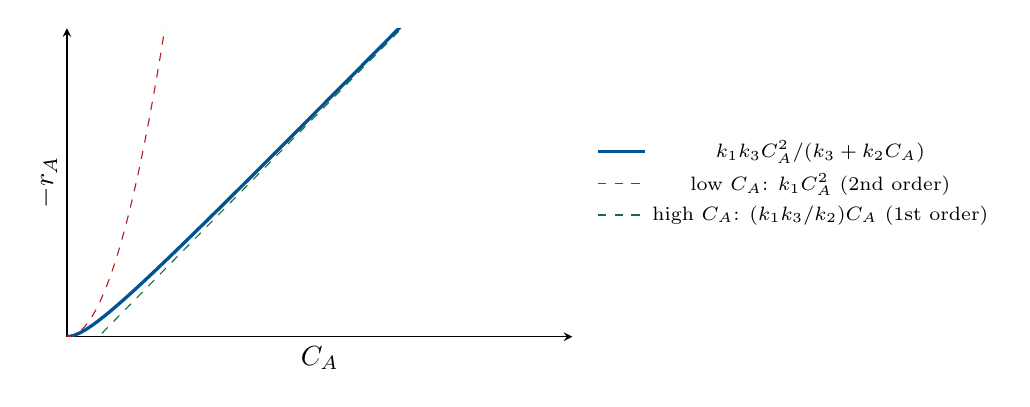
\begin{tikzpicture}
\begin{axis}[width=8cm,height=5.5cm,xmin=0,xmax=10,ymin=0,ymax=6,
  xlabel={$C_A$},ylabel={$-r_A$},axis lines=left,ticks=none,
  legend style={font=\scriptsize,at={(1.03,0.5)},anchor=west,draw=none,fill=none}]
\addplot[very thick,keyblue,domain=0:10,samples=80]{1*x^2/(1+1.6*x)*1.6};
\addlegendentry{$k_1k_3C_A^2/(k_3+k_2C_A)$}
\addplot[dashed,warnred,domain=0:2.0,samples=40]{1.6*x^2};
\addlegendentry{low $C_A$: $k_1C_A^2$ (2nd order)}
\addplot[dashed,tipgreen,domain=0:10]{x-0.625};
\addlegendentry{high $C_A$: $(k_1k_3/k_2)C_A$ (1st order)}
\end{axis}
\end{tikzpicture}
\end{center}

\subsection{Why do so many reactions look elementary? (Collision with an inert)}
If the activating partner is an inert $I$ (or the solvent) instead of A:
\[
\text{(1) } A+I\rxn{k_1}A^*+I\qquad
\text{(2) } A^*+I\rxn{k_2}A+I\qquad
\text{(3) } A^*\rxn{k_3}B+C
\]
PSSH: $k_1C_AC_I-k_2C_IC_{A^*}-k_3C_{A^*}=0\;\Rightarrow\;C_{A^*}=\dfrac{k_1C_AC_I}{k_3+k_2C_I}$, so
\[
-r_A=k_3C_{A^*}=\frac{k_1k_3C_AC_I}{k_3+k_2C_I}=\frac{kC_AC_I}{1+k'C_I}.
\]
When $C_I$ is large and essentially constant ($k_2C_I\gg k_3$), this becomes $-r_A=\dfrac{k_1k_3}{k_2}C_A$, i.e.\ \textbf{first order},
which looks exactly like an elementary rate law.
\begin{mistake}[Slide typos]
One slide prints the target as $-r_A=kC_A/(1+k'C_I)$ (missing $C_I$ in the numerator), and another prints the
denominator as ``$k_2+k_2C_I$''. The correct result is $\dfrac{k_1k_3C_AC_I}{k_3+k_2C_I}$.
\end{mistake}

\subsection{Rate that decreases with temperature: \ce{2NO + O2 -> 2NO2}}
\textbf{Observation:} the rate law is $r_{\mathrm{NO_2}}=k_{\mathrm{NO_2}}C_{\mathrm{NO}}^2C_{\mathrm{O_2}}$ (it looks
third-order elementary), but the rate \textbf{decreases} as $T$ increases. A true elementary step cannot do that,
because its $E>0$.

\textbf{Mechanism:}
\[
\text{(1) }\ce{NO + O2 ->[k_1] NO3^*}\qquad
\text{(2) }\ce{NO3^* ->[k_2] NO + O2}\qquad
\text{(3) }\ce{NO3^* + NO ->[k_3] 2NO2}
\]
\step{1}\textbf{Rates for each step} ($k_1,k_2$ w.r.t.\ NO; $k_3$ w.r.t.\ NO$_2$):
\[
r_{1,\mathrm{NO}}=-k_1C_{\mathrm{NO}}C_{\mathrm{O_2}},\quad
r_{2,\mathrm{NO}}=k_2C_{\mathrm{NO_3^*}},\quad
r_{3,\mathrm{NO_2}}=k_3C_{\mathrm{NO_3^*}}C_{\mathrm{NO}}.
\]
\step{2}\textbf{Convert each to NO$_3^*$:}
$r_{1,\mathrm{NO_3^*}}=-r_{1,\mathrm{NO}}=k_1C_{\mathrm{NO}}C_{\mathrm{O_2}}$;\;
$r_{2,\mathrm{NO_3^*}}=-r_{2,\mathrm{NO}}=-k_2C_{\mathrm{NO_3^*}}$;\;
$r_{3,\mathrm{NO_3^*}}=-\tfrac12r_{3,\mathrm{NO_2}}=-\tfrac{k_3}{2}C_{\mathrm{NO_3^*}}C_{\mathrm{NO}}$.

\step{3}\textbf{PSSH on NO$_3^*$:}
\[
k_1C_{\mathrm{NO}}C_{\mathrm{O_2}}-k_2C_{\mathrm{NO_3^*}}-\frac{k_3}{2}C_{\mathrm{NO_3^*}}C_{\mathrm{NO}}=0
\;\Rightarrow\;
C_{\mathrm{NO_3^*}}=\frac{k_1C_{\mathrm{NO}}C_{\mathrm{O_2}}}{k_2+\frac{k_3}{2}C_{\mathrm{NO}}}.
\]
\step{4}\textbf{Approximation.} NO$_3^*$ is very unstable, so it falls apart (step 2) much faster than it meets an NO
molecule: $k_2\gg\frac{k_3}{2}C_{\mathrm{NO}}$. Then $C_{\mathrm{NO_3^*}}\approx\dfrac{k_1}{k_2}C_{\mathrm{NO}}C_{\mathrm{O_2}}$
(steps 1 and 2 are effectively at equilibrium, $K_1=k_1/k_2$).

\step{5}\textbf{Rate of NO$_2$ formation:}
\[
r_{\mathrm{NO_2}}=k_3C_{\mathrm{NO_3^*}}C_{\mathrm{NO}}=\frac{k_1k_3}{k_2}C_{\mathrm{NO}}^2C_{\mathrm{O_2}}
\quad\Rightarrow\quad k_{\mathrm{NO_2}}=\frac{k_1k_3}{k_2}.
\]
\textbf{Why the rate falls with $T$:} each $k_i=A_ie^{-E_i/RT}$, so
\[
k_{\mathrm{NO_2}}=\frac{A_1A_3}{A_2}\exp\!\left[-\frac{E_1+E_3-E_2}{RT}\right],\qquad
E_{\text{app}}=E_1+E_3-E_2 .
\]
If the decomposition barrier $E_2$ is larger than $E_1+E_3$, then $E_{\text{app}}<0$ and the rate \textbf{decreases} with $T$.
Physically, a higher $T$ destroys NO$_3^*$ (step 2) faster than it speeds up the steps that use it.

\begin{center}
\begin{tikzpicture}
\begin{axis}[width=7cm,height=4.6cm,xmin=0,xmax=10,ymin=0,ymax=1.1,
  xlabel={$T$},ylabel={$-r_{\mathrm{NO_2}}$},axis lines=left,ticks=none]
\addplot[very thick,keyblue,domain=0.5:10,samples=60]{0.25+0.8*exp(-0.45*x)};
\end{axis}
\end{tikzpicture}
\end{center}

\begin{keyresult}[Apparent activation energy]
If $k_{\text{app}}=\dfrac{\prod k_{\text{num}}}{\prod k_{\text{den}}}$, then
$E_{\text{app}}=\sum E_{\text{num}}-\sum E_{\text{den}}$. It can be negative.
\end{keyresult}

\subsection{Seven steps to find (or check) a mechanism}
\begin{enumerate}
\item Assume one or more active intermediates.
\item Postulate a mechanism, using the rate law as a guide (denominator species collide with the intermediate).
\item Model each step as an \textbf{elementary} reaction.
\item Write the rate law for each step.
\item Apply the PSSH to each intermediate.
\item Eliminate the intermediate concentrations ($C_{A^*}$, $C_{\mathrm{H}\bullet}$, \ldots).
\item Compare with the experimental data (check limits, orders and the sign of $E_{\text{app}}$).
\end{enumerate}

% =====================================================================
\section{Lecture 7 (Part 1): Chain Reactions, \ce{H2 + Br2 -> 2HBr}}
% =====================================================================
\fogler{3rd ed.\ \S7.1; HW3 Problem 2}

\textbf{Observed rate law:}
\[
r_{\mathrm{HBr}}=\frac{k'C_{\mathrm{H_2}}C_{\mathrm{Br_2}}^{3/2}}{C_{\mathrm{Br_2}}+k''C_{\mathrm{HBr}}}.
\]
\textbf{Clues:} the fractional order $\tfrac32$ suggests Br$_2$ splits into two radicals (initiation). HBr in the
denominator means HBr attacks an intermediate (inhibition by product). The intermediates are H$\bullet$ and Br$\bullet$.

\subsection{Mechanism}
\begin{minipage}{0.52\textwidth}
\begin{tabular}{@{}lll@{}}
Initiation & \ce{Br2 ->[k_1] 2Br$\bullet$} & (1)\\[2pt]
Propagation & \ce{Br$\bullet$ + H2 ->[k_2] HBr + H$\bullet$} & (2)\\[2pt]
Propagation & \ce{H$\bullet$ + Br2 ->[k_3] HBr + Br$\bullet$} & (3)\\[2pt]
Inhibition & \ce{H$\bullet$ + HBr ->[k_4] H2 + Br$\bullet$} & (4)\\[2pt]
Termination & \ce{2Br$\bullet$ ->[k_5] Br2} & (5)
\end{tabular}
\end{minipage}\hfill
\begin{minipage}{0.44\textwidth}
\centering
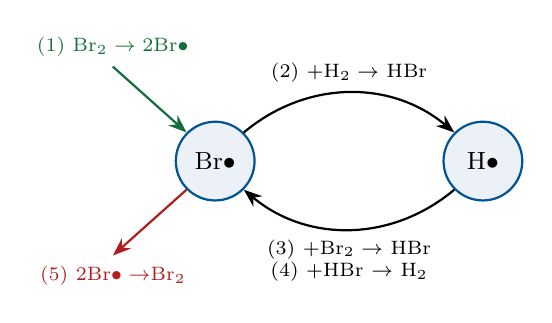
\begin{tikzpicture}[
  rad/.style={circle,draw=keyblue,fill=keyblue!8,thick,minimum size=10mm,font=\small}]
\node[rad] (br) at (0,0) {Br$\bullet$};
\node[rad] (h) at (3.4,0) {H$\bullet$};
\draw[-{Stealth},thick] (br.north east) to[bend left=40] node[above,font=\scriptsize]{(2) $+$H$_2\to$ HBr} (h.north west);
\draw[-{Stealth},thick] (h.south west) to[bend left=40] node[below,font=\scriptsize,align=center]{(3) $+$Br$_2\to$ HBr\\(4) $+$HBr $\to$ H$_2$} (br.south east);
\draw[-{Stealth},thick,tipgreen] (-1.3,1.2) node[above,font=\scriptsize]{(1) Br$_2\to2$Br$\bullet$} -- (br.north west);
\draw[-{Stealth},thick,warnred] (br.south west) -- (-1.3,-1.2) node[below,font=\scriptsize]{(5) 2Br$\bullet\to$Br$_2$};
\end{tikzpicture}

{\scriptsize Propagation is a cycle: each loop makes 2 HBr and gives back Br$\bullet$.}
\end{minipage}

Here $k_1$ is w.r.t.\ Br$_2$, $k_5$ is w.r.t.\ Br$\bullet$ (so $r_{5,\mathrm{Br}\bullet}=-k_5C_{\mathrm{Br}\bullet}^2$), and $k_2$--$k_4$ are
w.r.t.\ HBr (or the radical, which is the same thing because every coefficient is 1).

\subsection{Derivation}
\step{1}\textbf{Net rate of HBr formation.} HBr is made in (2) and (3) and consumed in (4):
\[
r_{\mathrm{HBr}}=k_2C_{\mathrm{Br}\bullet}C_{\mathrm{H_2}}+k_3C_{\mathrm{H}\bullet}C_{\mathrm{Br_2}}-k_4C_{\mathrm{H}\bullet}C_{\mathrm{HBr}}. \tag{i}
\]
We need $C_{\mathrm{H}\bullet}$ and $C_{\mathrm{Br}\bullet}$.

\step{2}\textbf{PSSH on H$\bullet$} (made in 2, used in 3 and 4):
\[
0=k_2C_{\mathrm{Br}\bullet}C_{\mathrm{H_2}}-k_3C_{\mathrm{H}\bullet}C_{\mathrm{Br_2}}-k_4C_{\mathrm{H}\bullet}C_{\mathrm{HBr}}
\;\Rightarrow\;
C_{\mathrm{H}\bullet}=\frac{k_2C_{\mathrm{Br}\bullet}C_{\mathrm{H_2}}}{k_3C_{\mathrm{Br_2}}+k_4C_{\mathrm{HBr}}}. \tag{ii}
\]
\step{3}\textbf{PSSH on Br$\bullet$} (made in 1, 3 and 4; used in 2 and 5):
\[
0=\underbrace{2k_1C_{\mathrm{Br_2}}}_{\text{(1), factor 2}}
\;\underbrace{-\,k_2C_{\mathrm{Br}\bullet}C_{\mathrm{H_2}}+k_3C_{\mathrm{H}\bullet}C_{\mathrm{Br_2}}+k_4C_{\mathrm{H}\bullet}C_{\mathrm{HBr}}}_{=\,0\text{ by the H}\bullet\text{ balance (ii)}}
\;-\;k_5C_{\mathrm{Br}\bullet}^2 .
\]
The middle group is exactly minus the H$\bullet$ balance, so it is zero. That leaves
\[
2k_1C_{\mathrm{Br_2}}=k_5C_{\mathrm{Br}\bullet}^2\;\Rightarrow\;
C_{\mathrm{Br}\bullet}=\left(\frac{2k_1}{k_5}\right)^{1/2}C_{\mathrm{Br_2}}^{1/2}. \tag{iii}
\]
In words: \emph{initiation and termination balance each other}. This is where the $\tfrac12$ order comes from.

\step{4}\textbf{Simplify (i) using (ii).} From the H$\bullet$ balance, $k_2C_{\mathrm{Br}\bullet}C_{\mathrm{H_2}}-k_4C_{\mathrm{H}\bullet}C_{\mathrm{HBr}}=k_3C_{\mathrm{H}\bullet}C_{\mathrm{Br_2}}$.
Substituting into (i):
\[
r_{\mathrm{HBr}}=2k_3C_{\mathrm{H}\bullet}C_{\mathrm{Br_2}}
=2k_3C_{\mathrm{Br_2}}\cdot\frac{k_2C_{\mathrm{Br}\bullet}C_{\mathrm{H_2}}}{k_3C_{\mathrm{Br_2}}+k_4C_{\mathrm{HBr}}}
=\frac{2k_2C_{\mathrm{Br}\bullet}C_{\mathrm{H_2}}C_{\mathrm{Br_2}}}{C_{\mathrm{Br_2}}+(k_4/k_3)C_{\mathrm{HBr}}}.
\]
(You can also substitute (ii) and (iii) straight into (i) and simplify; the result is the same, with more algebra.)

\step{5}\textbf{Insert (iii):}
\[
\boxed{\,r_{\mathrm{HBr}}=\frac{2k_2\left(\dfrac{2k_1}{k_5}\right)^{1/2}C_{\mathrm{H_2}}C_{\mathrm{Br_2}}^{3/2}}{C_{\mathrm{Br_2}}+(k_4/k_3)C_{\mathrm{HBr}}}
=\left(\frac{8k_1k_2^2}{k_5}\right)^{1/2}\frac{C_{\mathrm{H_2}}C_{\mathrm{Br_2}}^{3/2}}{C_{\mathrm{Br_2}}+(k_4/k_3)C_{\mathrm{HBr}}}\,}
\]
so $k'=2k_2\sqrt{2k_1/k_5}$ and $k''=k_4/k_3$. This matches the experiment. \checkmark

\subsection{The rate order changes with conditions}
\begin{center}
\renewcommand{\arraystretch}{1.3}
\begin{tabular}{lll}
\toprule
Condition & Dominant denominator term & Apparent rate law \\
\midrule
Start of reaction (no HBr yet) & $C_{\mathrm{Br_2}}$ & $r_{\mathrm{HBr},0}=k'C_{\mathrm{H_2}}C_{\mathrm{Br_2}}^{1/2}$ \\
High $C_{\mathrm{Br_2}}$ ($C_{\mathrm{Br_2}}\gg k''C_{\mathrm{HBr}}$) & $C_{\mathrm{Br_2}}$ & $\propto C_{\mathrm{H_2}}C_{\mathrm{Br_2}}^{1/2}$ \\
High $C_{\mathrm{HBr}}$ / low $C_{\mathrm{Br_2}}$ & $k''C_{\mathrm{HBr}}$ & $\propto C_{\mathrm{H_2}}C_{\mathrm{Br_2}}^{3/2}C_{\mathrm{HBr}}^{-1}$ \\
\bottomrule
\end{tabular}
\end{center}

\begin{examtip}
For a chain mechanism, add the PSSH equations for all radicals: the propagation steps cancel, and you are left with
\textbf{rate of initiation = rate of termination}. That gives the radical concentration almost for free.
\end{examtip}

% =====================================================================
\section{Lecture 7 (Part 2): Enzyme Kinetics}
% =====================================================================
\fogler{3rd ed.\ \S7.4--7.5; slides cite pp.~401--409, Ex.~7-3}

\subsection{Fundamentals}
\begin{itemize}
\item Enzymes are protein catalysts. They give the substrate S a \textbf{faster pathway} to the product P through an
enzyme--substrate complex E$\cdot$S, and the enzyme is regenerated.
\item They are highly \textbf{specific}: a given enzyme catalyses essentially one reaction. Example: urease
decomposes urea only, \ce{NH2CONH2 + urease ->[H2O] 2NH3 + CO2 + urease}.
\end{itemize}
\begin{center}
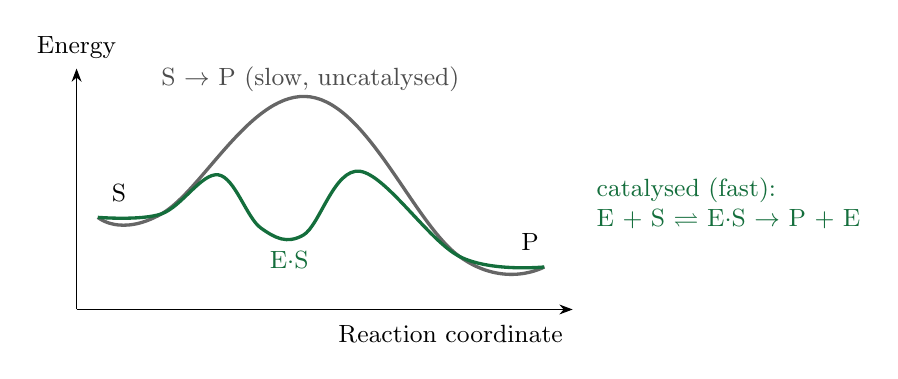
\begin{tikzpicture}[scale=0.9]
\draw[-{Stealth}] (0,0)--(0,3.4) node[above]{\small Energy};
\draw[-{Stealth}] (0,0)--(7,0) node[below left,yshift=-2pt]{\small Reaction coordinate};
\draw[very thick,black!60] plot[smooth,tension=0.7] coordinates{(0.3,1.3)(1.2,1.35)(3.3,3.0)(5.4,0.75)(6.6,0.6)};
\node[font=\small,black!70] at (3.3,3.25) {S $\to$ P (slow, uncatalysed)};
\draw[very thick,tipgreen] plot[smooth,tension=0.6] coordinates{(0.3,1.3)(1.2,1.35)(2.0,1.9)(2.6,1.15)(3.2,1.05)(4.0,1.95)(5.4,0.75)(6.6,0.6)};
\node[font=\small,tipgreen] at (3.0,0.7) {E$\cdot$S};
\node[font=\small,tipgreen,align=left,anchor=west] at (7.2,1.5) {catalysed (fast):\\E + S $\rightleftharpoons$ E$\cdot$S $\to$ P + E};
\node[font=\small] at (0.6,1.65) {S};
\node[font=\small] at (6.4,0.95) {P};
\end{tikzpicture}
\end{center}

\subsection{Michaelis--Menten derivation (urease mechanism)}
\textbf{Mechanism} (W = water, always in large excess):
\[
\text{(1) } E+S\rxn{k_1}E\cdot S\qquad
\text{(2) } E\cdot S\rxn{k_2}E+S\qquad
\text{(3) } E\cdot S+W\rxn{k_3}P+E
\]
\textbf{Enzyme balance} (the enzyme is either free or complexed): $C_{E,t}=C_E+C_{E\cdot S}$.

\step{1}\textbf{Rate of product formation:} $r_P=k_3C_{E\cdot S}C_W$. \quad $C_{E\cdot S}$ is not measurable.

\step{2}\textbf{PSSH on E$\cdot$S:}
\[
r_{E\cdot S}=k_1C_EC_S-k_2C_{E\cdot S}-k_3C_{E\cdot S}C_W=0 .
\]
\step{3}\textbf{Eliminate the free enzyme} using $C_E=C_{E,t}-C_{E\cdot S}$:
\[
k_1(C_{E,t}-C_{E\cdot S})C_S=C_{E\cdot S}(k_2+k_3C_W)
\;\Rightarrow\;
C_{E\cdot S}=\frac{k_1C_{E,t}C_S}{k_1C_S+k_2+k_3C_W}.
\]
\step{4}\textbf{Substitute:}
\[
r_P=\frac{k_1k_3C_{E,t}C_WC_S}{k_1C_S+k_2+k_3C_W}.
\]
\step{5}\textbf{Group constants.} Divide the top and bottom by $k_1$, and define
\[
k_{\text{cat}}=k_3'=k_3C_W\ \text{(turnover number)},\qquad
K_M=\frac{k_2+k_3'}{k_1}\ \text{(Michaelis constant)},\qquad
V_{\max}=k_{\text{cat}}C_{E,t}.
\]
\begin{keyresult}[Michaelis--Menten equation]
\[
-r_S=r_P=\frac{V_{\max}C_S}{K_M+C_S}=\frac{k_{\text{cat}}C_{E,t}C_S}{K_M+C_S}
\]
\begin{itemize}
\item $C_S\ll K_M$: $-r_S\approx\dfrac{V_{\max}}{K_M}C_S$, \textbf{first order}.
\item $C_S\gg K_M$: $-r_S\approx V_{\max}$, \textbf{zero order} (the enzyme is saturated).
\item At $C_S=K_M$: $-r_S=V_{\max}/2$. \textbf{$K_M$ is the substrate concentration at half the maximum rate}
(set $\frac{V_{\max}}{2}=\frac{V_{\max}S_{1/2}}{K_M+S_{1/2}}$, which gives $K_M=S_{1/2}$).
A small $K_M$ means a high affinity of the enzyme for S.
\end{itemize}
\end{keyresult}

\textbf{Turnover number} $k_{\text{cat}}$: the number of substrate molecules converted per enzyme molecule per unit time
(molecules/molecule/s). Example: catalase, \ce{H2O2 + E -> H2O + O + E}, has $k_{\text{cat}}=4\times10^{7}$~s$^{-1}$.

\begin{center}
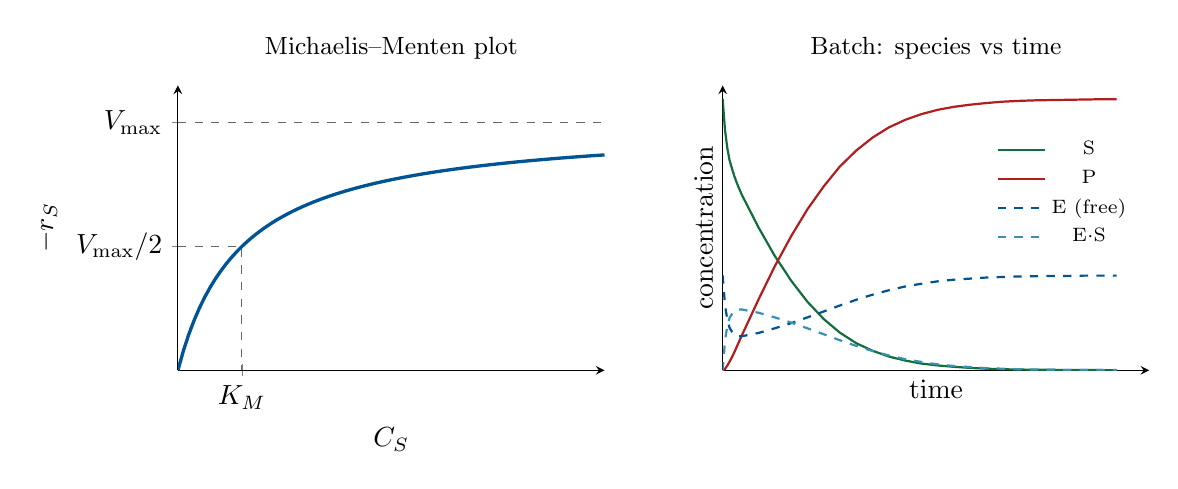
\begin{tikzpicture}
\begin{axis}[name=mm,width=7cm,height=5.2cm,xmin=0,xmax=10,ymin=0,ymax=1.15,
  xlabel={$C_S$},ylabel={$-r_S$},axis lines=left,xtick={1.5},xticklabels={$K_M$},
  ytick={0.5,1},yticklabels={$V_{\max}/2$,$V_{\max}$},title={\small Michaelis--Menten plot}]
\addplot[very thick,keyblue,domain=0:10,samples=80]{x/(1.5+x)};
\addplot[dashed,black!60] coordinates{(0,1)(10,1)};
\addplot[dashed,black!60] coordinates{(0,0.5)(1.5,0.5)(1.5,0)};
\end{axis}
\begin{axis}[at={(mm.east)},anchor=west,xshift=1.5cm,width=7cm,height=5.2cm,
  xmin=0,xmax=13,ymin=0,ymax=1.05,xlabel={time},ylabel={concentration},axis lines=left,ticks=none,
  title={\small Batch: species vs time},legend style={font=\scriptsize,draw=none,fill=none,at={(0.98,0.62)},anchor=east}]
\addplot[thick,tipgreen] coordinates{(0.00,1.000) (0.07,0.887) (0.14,0.820) (0.21,0.774) (0.29,0.741) (0.36,0.714) (0.43,0.691) (0.50,0.670) (0.60,0.643) (1.10,0.525) (1.59,0.421) (2.09,0.330) (2.58,0.253) (3.08,0.189) (3.57,0.139) (4.07,0.100) (4.57,0.072) (5.06,0.051) (5.56,0.036) (6.05,0.025) (6.55,0.018) (7.04,0.013) (7.54,0.009) (8.03,0.006) (8.53,0.004) (9.03,0.003) (9.52,0.002) (10.02,0.002) (10.51,0.001) (11.01,0.001) (11.50,0.001) (12.00,0.000)};
\addlegendentry{S}
\addplot[thick,warnred] coordinates{(0.00,0.000) (0.07,0.005) (0.14,0.017) (0.21,0.032) (0.29,0.050) (0.36,0.068) (0.43,0.087) (0.50,0.106) (0.60,0.133) (1.10,0.263) (1.59,0.384) (2.09,0.495) (2.58,0.593) (3.08,0.678) (3.57,0.751) (4.07,0.810) (4.57,0.858) (5.06,0.895) (5.56,0.923) (6.05,0.944) (6.55,0.960) (7.04,0.971) (7.54,0.979) (8.03,0.985) (8.53,0.990) (9.03,0.993) (9.52,0.995) (10.02,0.996) (10.51,0.997) (11.01,0.998) (11.50,0.999) (12.00,0.999)};
\addlegendentry{P}
\addplot[thick,dashed,keyblue] coordinates{(0.00,0.350) (0.07,0.242) (0.14,0.187) (0.21,0.157) (0.29,0.141) (0.36,0.132) (0.43,0.128) (0.50,0.126) (0.60,0.126) (1.10,0.138) (1.59,0.155) (2.09,0.174) (2.58,0.195) (3.08,0.217) (3.57,0.239) (4.07,0.260) (4.57,0.279) (5.06,0.295) (5.56,0.309) (6.05,0.319) (6.55,0.328) (7.04,0.334) (7.54,0.338) (8.03,0.342) (8.53,0.344) (9.03,0.346) (9.52,0.347) (10.02,0.348) (10.51,0.348) (11.01,0.349) (11.50,0.349) (12.00,0.349)};
\addlegendentry{E (free)}
\addplot[thick,dashed,cyan!70!black] coordinates{(0.00,0.000) (0.07,0.108) (0.14,0.163) (0.21,0.193) (0.29,0.209) (0.36,0.218) (0.43,0.222) (0.50,0.224) (0.60,0.224) (1.10,0.212) (1.59,0.195) (2.09,0.176) (2.58,0.155) (3.08,0.133) (3.57,0.111) (4.07,0.090) (4.57,0.071) (5.06,0.055) (5.56,0.041) (6.05,0.031) (6.55,0.022) (7.04,0.016) (7.54,0.012) (8.03,0.008) (8.53,0.006) (9.03,0.004) (9.52,0.003) (10.02,0.002) (10.51,0.001) (11.01,0.001) (11.50,0.001) (12.00,0.001)};
\addlegendentry{E$\cdot$S}
\end{axis}
\end{tikzpicture}
\end{center}
{\small Right: $C_{E}+C_{E\cdot S}=C_{E,t}$ at all times. After a very short start-up, $C_{E\cdot S}$ changes slowly
compared with S and P, which is why the PSSH works.}

\subsection{Finding $V_{\max}$ and $K_M$ from data: linearised plots}
\textbf{Lineweaver--Burk (double reciprocal).} Invert the M--M equation:
\[
\frac{1}{-r_S}=\frac{K_M+C_S}{V_{\max}C_S}=\frac{1}{V_{\max}}+\frac{K_M}{V_{\max}}\cdot\frac{1}{C_S}.
\]
Plot $1/(-r_S)$ against $1/C_S$: a straight line with \textbf{intercept $1/V_{\max}$}, \textbf{slope $K_M/V_{\max}$}, and
\textbf{$x$-intercept $-1/K_M$}. Then $V_{\max}=1/\text{intercept}$ and $K_M=\text{slope}\times V_{\max}$.

\begin{center}
\begin{tikzpicture}
\begin{axis}[width=8cm,height=5.6cm,axis lines=middle,xmin=-0.9,xmax=2.6,ymin=-0.45,ymax=3.4,
  xlabel={$\dfrac{1}{C_S}$},ylabel={$\dfrac{1}{-r_S}$},ticks=none,
  xlabel style={anchor=north east},ylabel style={anchor=south}]
\addplot[dashed,thick,keyblue,domain=-0.6:2.4]{1+1.6*x};
\addplot[only marks,mark=*,mark size=1.6pt] coordinates{(0.25,1.43)(0.5,1.78)(0.9,2.46)(1.4,3.22)(0.15,1.22)};
\node[font=\scriptsize,anchor=south east] at (axis cs:-0.05,1.0) {$1/V_{\max}$};
\node[font=\scriptsize,anchor=north] at (axis cs:-0.625,-0.02) {$-1/K_M$};
\draw[thick] (axis cs:1.0,2.6)--(axis cs:1.6,2.6)--(axis cs:1.6,3.56);
\node[font=\scriptsize,anchor=west] at (axis cs:1.62,2.95) {slope $=K_M/V_{\max}$};
\end{axis}
\end{tikzpicture}
\end{center}

Two other linear forms (Fogler) are less sensitive to errors in the low-$C_S$ points, which dominate a
Lineweaver--Burk plot:
\begin{itemize}
\item \textbf{Hanes--Woolf:} $\dfrac{C_S}{-r_S}=\dfrac{K_M}{V_{\max}}+\dfrac{1}{V_{\max}}C_S$ \quad(plot $C_S/(-r_S)$ vs $C_S$).
\item \textbf{Eadie--Hofstee:} $-r_S=V_{\max}-K_M\dfrac{-r_S}{C_S}$ \quad(plot $-r_S$ vs $-r_S/C_S$; slope $=-K_M$).
\end{itemize}

\subsection{Enzyme reactions in a batch reactor (very exam-friendly)}
Mole balance, constant volume: $\dfrac{dC_S}{dt}=r_S=-\dfrac{V_{\max}C_S}{K_M+C_S}$.

\step{1}Separate variables: $\displaystyle -\frac{K_M+C_S}{C_S}\,dC_S=V_{\max}\,dt$.

\step{2}Integrate from $C_{S0}$ at $t=0$ to $C_S$ at $t$:
$\displaystyle K_M\ln\frac{C_{S0}}{C_S}+(C_{S0}-C_S)=V_{\max}\,t$.

\step{3}With $C_S=C_{S0}(1-X)$:
\begin{keyresult}[Batch enzymatic reactor]
\[
t=\frac{K_M}{V_{\max}}\ln\frac{1}{1-X}+\frac{C_{S0}X}{V_{\max}}
\]
The first term is the first-order (low-$C_S$) part and the second is the zero-order (saturated) part.
Rearranged for data analysis: $\dfrac{1}{t}\ln\dfrac{C_{S0}}{C_S}=\dfrac{V_{\max}}{K_M}-\dfrac{C_{S0}-C_S}{K_M\,t}$.
\end{keyresult}
\textbf{CSTR:} $V=\dfrac{v_0(C_{S0}-C_S)}{-r_S}=\dfrac{v_0(C_{S0}-C_S)(K_M+C_S)}{V_{\max}C_S}$.

% ---------------------------------------------------------------------
\subsection{Enzyme inhibition}
An inhibitor I binds the enzyme and makes it inactive. There are three types:
\begin{center}
\renewcommand{\arraystretch}{1.3}
\begin{tabular}{l p{6.4cm} l}
\toprule
Type & Inhibitor binds to & Inactive complex(es) \\
\midrule
1. Competitive & free enzyme only (competes with S for the active site) & \ce{E + I <=> I.E} \\
2. Uncompetitive & the E$\cdot$S complex only & \ce{E.S + I <=> I.E.S} \\
3. Noncompetitive & both E and E$\cdot$S (binds a different site) & \ce{E + I <=> I.E}\\
 & & \ce{E.S + I <=> I.E.S}\\
 & & \ce{I.E + S <=> I.E.S}\\
\bottomrule
\end{tabular}
\end{center}
In all three, use the same recipe: (1) PSSH or equilibrium for each complex; (2) express every complex in terms of $C_E$;
(3) total enzyme balance to find $C_E$; (4) $-r_S=r_P=k_3C_{E\cdot S}$; (5) invert for the Lineweaver--Burk form.
Throughout, $K_M=\dfrac{k_2+k_3}{k_1}$ (water folded into $k_3$) and $V_{\max}=k_3C_{E,t}$.

\subsubsection*{1. Competitive inhibition (derived in lecture)}
\[
E+S\underset{k_2}{\overset{k_1}{\rightleftharpoons}}E\cdot S\rxn{k_3}E+P,\qquad
E+I\underset{k_5}{\overset{k_4}{\rightleftharpoons}}E\cdot I\ \text{(inactive)}
\]
\step{1}PSSH on E$\cdot$S: $0=k_1C_SC_E-(k_2+k_3)C_{E\cdot S}\Rightarrow C_{E\cdot S}=\dfrac{C_SC_E}{K_M}$.

\step{2}PSSH on E$\cdot$I: $0=k_4C_IC_E-k_5C_{E\cdot I}\Rightarrow C_{E\cdot I}=\dfrac{C_IC_E}{K_I}$, with $K_I=\dfrac{k_5}{k_4}$.

\step{3}Total enzyme:
$C_{E,t}=C_E+C_{E\cdot S}+C_{E\cdot I}=C_E\left(1+\dfrac{C_S}{K_M}+\dfrac{C_I}{K_I}\right)$.

\step{4}Rate:
\[
-r_S=k_3C_{E\cdot S}=\frac{k_3C_SC_E}{K_M}=\frac{k_3C_{E,t}C_S/K_M}{1+\frac{C_S}{K_M}+\frac{C_I}{K_I}}
=\frac{V_{\max}C_S}{C_S+K_M\left(1+\frac{C_I}{K_I}\right)}.
\]
\step{5}Invert:
$\displaystyle\frac{1}{-r_S}=\frac{1}{V_{\max}}+\frac{K_M}{V_{\max}}\left(1+\frac{C_I}{K_I}\right)\frac{1}{C_S}$.

\textbf{Meaning:} the intercept ($1/V_{\max}$) is unchanged and the slope increases. The apparent $K_M$ becomes
$K_M(1+C_I/K_I)$. At a very high $C_S$ the substrate out-competes the inhibitor, so $V_{\max}$ can still be reached.

\subsubsection*{2. Uncompetitive inhibition}
\[
E+S\rightleftharpoons E\cdot S\rxn{k_3}E+P,\qquad
E\cdot S+I\underset{k_5}{\overset{k_4}{\rightleftharpoons}}I\cdot E\cdot S\ \text{(inactive)}
\]
\step{1}PSSH on E$\cdot$S. The I-binding step is at equilibrium, so its net rate is zero and it drops out of the E$\cdot$S balance:
$C_{E\cdot S}=\dfrac{C_SC_E}{K_M}$.

\step{2}PSSH on I$\cdot$E$\cdot$S: $0=k_4C_IC_{E\cdot S}-k_5C_{I\cdot E\cdot S}\Rightarrow C_{I\cdot E\cdot S}=\dfrac{C_IC_{E\cdot S}}{K_I}=\dfrac{C_IC_SC_E}{K_IK_M}$.

\step{3}Total enzyme:
\[
C_{E,t}=C_E+C_{E\cdot S}+C_{I\cdot E\cdot S}=C_E\left[1+\frac{C_S}{K_M}\left(1+\frac{C_I}{K_I}\right)\right].
\]
\step{4}Rate (multiply the top and bottom by $K_M$):
\[
-r_S=\frac{k_3C_SC_E}{K_M}=\frac{V_{\max}C_S}{K_M+C_S\left(1+\frac{C_I}{K_I}\right)}.
\]
\step{5}Invert:
\[
\frac{1}{-r_S}=\frac{K_M+C_S(1+C_I/K_I)}{V_{\max}C_S}
=\frac{1}{V_{\max}}\left(1+\frac{C_I}{K_I}\right)+\frac{K_M}{V_{\max}}\cdot\frac{1}{C_S}.
\]
\textbf{Meaning:} the slope is unchanged and the intercept increases, so the lines are \textbf{parallel}.
Both the apparent $V_{\max}$ and the apparent $K_M$ are divided by $(1+C_I/K_I)$.

\subsubsection*{3. Noncompetitive inhibition (HW3 Problem 3)}
I binds to a site different from the active site, so it can attach to free E or to E$\cdot$S, and S can still bind to I$\cdot$E:
\[
\begin{aligned}
&E+S\rightleftharpoons E\cdot S\rxn{k_3}E+P, \qquad
E+I\rightleftharpoons I\cdot E\ (K_I),\\
&E\cdot S+I\rightleftharpoons I\cdot E\cdot S\ (K_I),\qquad
I\cdot E+S\rightleftharpoons I\cdot E\cdot S\ (\text{inactive}).
\end{aligned}
\]
Assume I binds equally well to E and E$\cdot$S (the same $K_I$), and that S binds I$\cdot$E as it binds E (the same $K_M$).

\step{1}Express every complex through $C_E$:
\[
C_{E\cdot S}=\frac{C_SC_E}{K_M},\qquad C_{I\cdot E}=\frac{C_IC_E}{K_I},\qquad
C_{I\cdot E\cdot S}=\frac{C_IC_{E\cdot S}}{K_I}=\frac{C_IC_SC_E}{K_IK_M}.
\]
\step{2}Total enzyme. The four terms factor neatly:
\[
C_{E,t}=C_E\left[1+\frac{C_S}{K_M}+\frac{C_I}{K_I}+\frac{C_IC_S}{K_IK_M}\right]
=C_E\left(1+\frac{C_S}{K_M}\right)\left(1+\frac{C_I}{K_I}\right).
\]
\step{3}Rate:
\[
-r_S=\frac{k_3C_SC_E}{K_M}=\frac{k_3C_{E,t}C_S}{K_M\left(1+\frac{C_S}{K_M}\right)\left(1+\frac{C_I}{K_I}\right)}
=\frac{V_{\max}C_S}{(C_S+K_M)\left(1+\frac{C_I}{K_I}\right)}.
\]
\step{4}Invert:
\[
\frac{1}{-r_S}=\frac{1}{V_{\max}}\left(1+\frac{C_I}{K_I}\right)+\frac{K_M}{V_{\max}}\left(1+\frac{C_I}{K_I}\right)\frac{1}{C_S}.
\]
\textbf{Meaning:} the slope and the intercept both increase by the same factor $(1+C_I/K_I)$. The $x$-intercept
($-1/K_M$) is unchanged, so the lines meet on the $x$-axis. The apparent $V_{\max}$ drops and $K_M$ stays the same.

\begin{center}
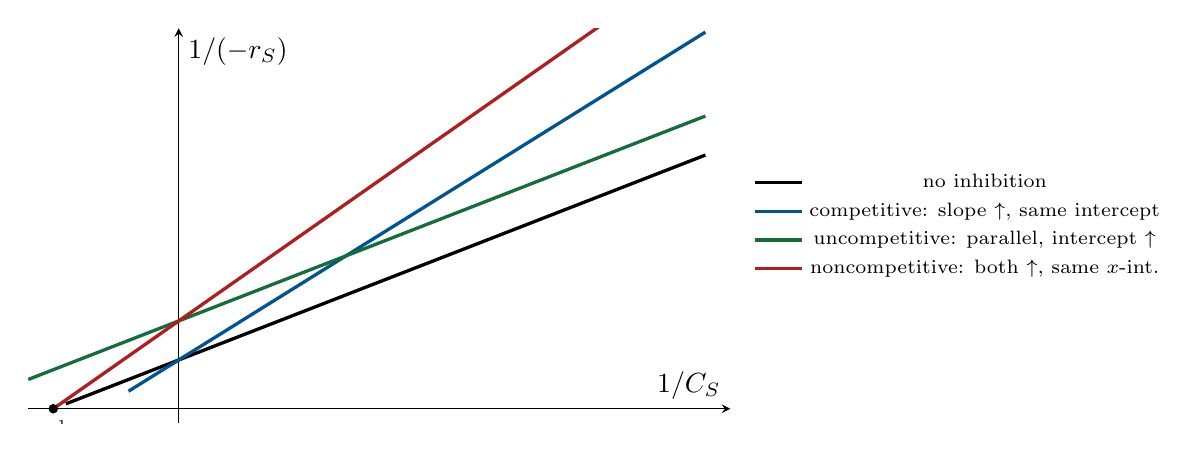
\begin{tikzpicture}
\begin{axis}[width=10.5cm,height=6.6cm,axis lines=middle,xmin=-0.6,xmax=2.2,ymin=-0.15,ymax=3.9,
  xlabel={$1/C_S$},ylabel={$1/(-r_S)$},ticks=none,
  legend style={font=\scriptsize,at={(1.02,0.5)},anchor=west,draw=none}]
\addplot[very thick,black,domain=-0.45:2.1]{0.5+1.0*x};\addlegendentry{no inhibition}
\addplot[very thick,keyblue,domain=-0.2:2.1]{0.5+1.6*x};\addlegendentry{competitive: slope $\uparrow$, same intercept}
\addplot[very thick,tipgreen,domain=-0.6:2.1]{0.9+1.0*x};\addlegendentry{uncompetitive: parallel, intercept $\uparrow$}
\addplot[very thick,warnred,domain=-0.5:2.0]{0.9+1.8*x};\addlegendentry{noncompetitive: both $\uparrow$, same $x$-int.}
\addplot[only marks,mark=*,mark size=1.5pt] coordinates{(-0.5,0)};
\node[font=\scriptsize,anchor=north] at (axis cs:-0.5,-0.02) {$-\frac{1}{K_M}$};
\end{axis}
\end{tikzpicture}
\end{center}

\begin{keyresult}[Inhibition summary: write $\phi=1+C_I/K_I$]
\renewcommand{\arraystretch}{1.5}
\begin{tabular}{llccc}
\toprule
Type & $-r_S$ & L--B intercept & L--B slope & apparent $V_{\max}$, $K_M$\\
\midrule
None & $\dfrac{V_{\max}C_S}{K_M+C_S}$ & $\dfrac{1}{V_{\max}}$ & $\dfrac{K_M}{V_{\max}}$ & $V_{\max}$, $K_M$\\
Competitive & $\dfrac{V_{\max}C_S}{C_S+K_M\phi}$ & same & $\times\phi$ & $V_{\max}$, $K_M\phi$\\
Uncompetitive & $\dfrac{V_{\max}C_S}{K_M+C_S\phi}$ & $\times\phi$ & same & $V_{\max}/\phi$, $K_M/\phi$\\
Noncompetitive & $\dfrac{V_{\max}C_S}{(C_S+K_M)\phi}$ & $\times\phi$ & $\times\phi$ & $V_{\max}/\phi$, $K_M$\\
\bottomrule
\end{tabular}
\end{keyresult}

\begin{examtip}
To identify the inhibition type from data: compute $1/(-r_S)$ and $1/C_S$ with and without inhibitor, fit both lines,
and compare the slopes and intercepts. The \emph{ratio} (inhibited/uninhibited) of whichever changed equals
$\phi=1+C_I/K_I$, so $K_I=C_I/(\phi-1)$.
\end{examtip}

% =====================================================================
\section{Lectures 8--9: Catalysis and Langmuir--Hinshelwood Kinetics}
% =====================================================================
\fogler{4th ed.\ Ch.~10, pp.~645--700; 5th ed.\ Ch.~10 (starts p.~399)}

\subsection{Catalysts and an industrial example}
\begin{itemize}
\item A \textbf{catalyst} changes the rate of a reaction (by giving a lower-energy pathway) without being consumed.
It does \textbf{not} change the equilibrium.
\item \textbf{Heterogeneous} catalysis: the catalyst is a solid and the reactants are gases or liquids. The reaction
happens on the \textbf{surface}, mostly inside the \textbf{pores} of a porous pellet, which is where nearly all of the area is.
\item A catalyst is often a small amount of \textbf{active} material (Pt, Ni, Fe\ldots) dispersed on a high-area
\textbf{support} (Al$_2$O$_3$, SiO$_2$, zeolites, carbon).
\end{itemize}

\textbf{Haber--Bosch ammonia synthesis} (\ce{N2 + 3H2 -> 2NH3}, promoted Fe catalyst with K$_2$O/Al$_2$O$_3$):

\begin{minipage}{0.42\textwidth}
\small
\begin{tabular}{@{}ll@{}}
(1) & \ce{N2(g) -> N2(ads)}\\
(2) & \ce{N2(ads) -> 2N(ads)}\\
(3) & \ce{H2(g) -> H2(ads)}\\
(4) & \ce{H2(ads) -> 2H(ads)}\\
(5) & \ce{N(ads) + 3H(ads) -> NH3(ads)}\\
(6) & \ce{NH3(ads) -> NH3(g)}
\end{tabular}

Adsorb, then dissociate, then react on the surface, then desorb.
\end{minipage}\hfill
\begin{minipage}{0.56\textwidth}
\centering
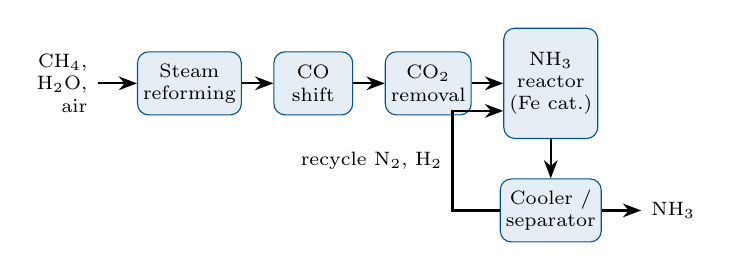
\begin{tikzpicture}[font=\scriptsize,
  u/.style={draw=keyblue,fill=keyblue!10,rounded corners,minimum height=8mm,minimum width=1.0cm,align=center,inner sep=2pt},
  a/.style={-{Stealth},thick}]
\node[u] (sr) {Steam\\reforming};
\node[u,right=4mm of sr] (sh) {CO\\shift};
\node[u,right=4mm of sh] (co) {CO$_2$\\removal};
\node[u,right=4mm of co,minimum height=14mm] (re) {NH$_3$\\reactor\\(Fe cat.)};
\node[u,below=5mm of re] (cl) {Cooler /\\separator};
\draw[a] ($(sr.west)+(-0.5,0)$) node[left,align=right]{CH$_4$,\\H$_2$O,\\air} -- (sr);
\draw[a] (sr)--(sh); \draw[a] (sh)--(co); \draw[a] (co)--(re);
\draw[a] (re)--(cl);
\draw[a] (cl.east) -- ++(0.5,0) node[right]{NH$_3$};
\draw[a] (cl.west) -- ++(-0.6,0) |- node[pos=0.25,left]{recycle N$_2$, H$_2$} ($(re.west)+(0,-0.35)$);
\end{tikzpicture}
\end{minipage}

\subsection{The seven steps of a heterogeneous catalytic reaction}
\fogler{4th ed.\ p.~656}

\begin{center}
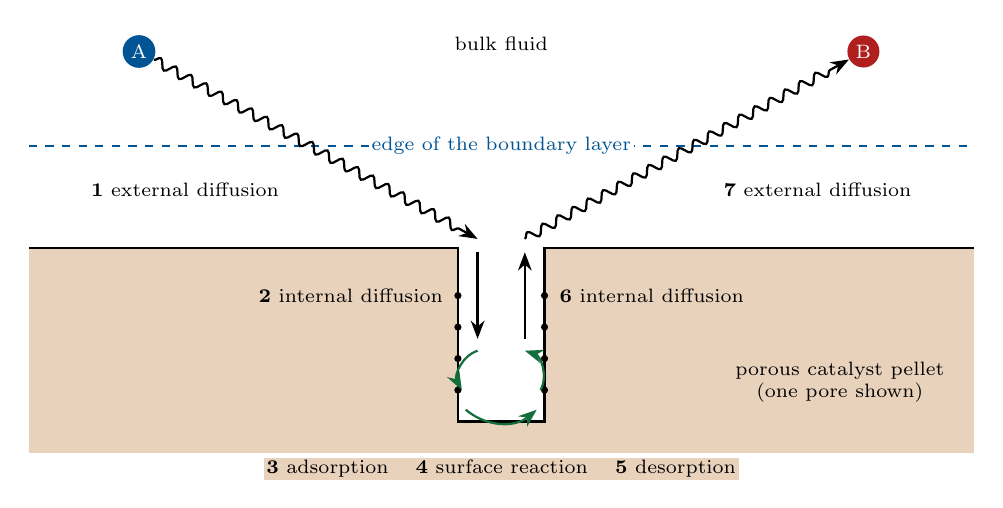
\begin{tikzpicture}[font=\small]
% pellet with one pore
\fill[brown!35] (-6,0) rectangle (-0.55,-2.6);
\fill[brown!35] (0.55,0) rectangle (6,-2.6);
\fill[brown!35] (-0.55,-2.2) rectangle (0.55,-2.6);
\draw[thick] (-6,0)--(-0.55,0)--(-0.55,-2.2)--(0.55,-2.2)--(0.55,0)--(6,0);
\node[font=\scriptsize,align=center] at (4.3,-1.7) {porous catalyst pellet\\(one pore shown)};
% active sites on pore wall
\foreach \y in {-0.6,-1.0,-1.4,-1.8}{\fill[black] (-0.55,\y) circle(1.3pt); \fill[black] (0.55,\y) circle(1.3pt);}
% boundary layer and bulk
\draw[dashed,thick,keyblue] (-6,1.3)--(6,1.3);
\node[font=\scriptsize,keyblue,fill=white,inner sep=1pt] at (0,1.3) {edge of the boundary layer};
\node[font=\scriptsize] at (0,2.6) {bulk fluid};
\node[circle,fill=keyblue,text=white,inner sep=1.5pt,font=\scriptsize] (A) at (-4.6,2.5) {A};
\node[circle,fill=warnred,text=white,inner sep=1.5pt,font=\scriptsize] (B) at (4.6,2.5) {B};
% 1 external diffusion of A
\draw[-{Stealth},thick,decorate,decoration={snake,amplitude=0.6mm,segment length=2.2mm,post length=2mm}] (A)--(-0.3,0.12);
\node[font=\scriptsize,anchor=east] at (-2.7,0.75) {\textbf{1} external diffusion};
% 2 internal diffusion
\draw[-{Stealth},thick] (-0.3,-0.05)--(-0.3,-1.15);
\node[font=\scriptsize,anchor=east,fill=brown!35,inner sep=1pt] at (-0.7,-0.6) {\textbf{2} internal diffusion};
% 3,4,5 on the wall
\draw[-{Stealth},thick,tipgreen] (-0.3,-1.3) to[bend right=50] (-0.5,-1.8);
\draw[-{Stealth},thick,tipgreen] (-0.45,-2.05) to[bend right=40] (0.45,-2.05);
\draw[-{Stealth},thick,tipgreen] (0.5,-1.8) to[bend right=50] (0.3,-1.3);
\node[font=\scriptsize,anchor=north,fill=brown!35,inner sep=1pt,align=center] at (0,-2.65) {\textbf{3} adsorption \;\; \textbf{4} surface reaction \;\; \textbf{5} desorption};
% 6 internal diffusion of B
\draw[-{Stealth},thick] (0.3,-1.15)--(0.3,-0.05);
\node[font=\scriptsize,anchor=west,fill=brown!35,inner sep=1pt] at (0.7,-0.6) {\textbf{6} internal diffusion};
% 7 external diffusion of B
\draw[-{Stealth},thick,decorate,decoration={snake,amplitude=0.6mm,segment length=2.2mm,post length=2mm}] (0.3,0.12)--(B);
\node[font=\scriptsize,anchor=west] at (2.7,0.75) {\textbf{7} external diffusion};
\end{tikzpicture}
\end{center}

\begin{enumerate}
\item \textbf{External diffusion} of A from the bulk, through the boundary layer, to the pellet surface.
\item \textbf{Internal diffusion} of A through the pores to the catalytic surface.
\item \textbf{Adsorption} of A onto a site: \ce{A + S <=> A.S}.
\item \textbf{Surface reaction}: \ce{A.S <=> B.S}.
\item \textbf{Desorption} of B: \ce{B.S <=> B + S}.
\item \textbf{Internal diffusion} of B to the pore mouth.
\item \textbf{External diffusion} of B to the bulk.
\end{enumerate}
At steady state all the steps run in series at the same rate. The \textbf{slowest} step controls the overall rate,
like the largest resistor in a series circuit. In Lectures 8--9 we assume diffusion (1, 2, 6, 7) is fast and focus on
steps 3--5 (\emph{reaction-limited}). Diffusion limitations come later in the course.

\begin{center}
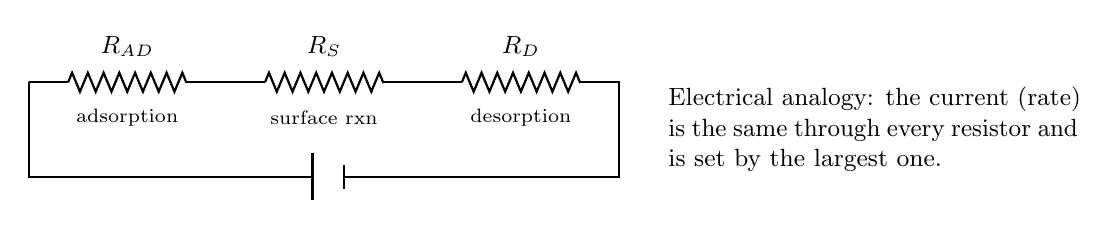
\begin{tikzpicture}[font=\small]
\draw[thick] (0,0) -- (0.5,0);
\draw[thick,decorate,decoration={zigzag,segment length=2mm,amplitude=1.2mm}] (0.5,0)--(2,0);
\draw[thick] (2,0)--(3,0);
\draw[thick,decorate,decoration={zigzag,segment length=2mm,amplitude=1.2mm}] (3,0)--(4.5,0);
\draw[thick] (4.5,0)--(5.5,0);
\draw[thick,decorate,decoration={zigzag,segment length=2mm,amplitude=1.2mm}] (5.5,0)--(7,0);
\draw[thick] (7,0)--(7.5,0)--(7.5,-1.2)--(4.0,-1.2);
\draw[thick] (3.6,-1.2)--(0,-1.2)--(0,0);
\draw[very thick] (3.6,-0.9)--(3.6,-1.5); \draw[thick] (4.0,-1.05)--(4.0,-1.35);
\node at (1.25,0.45) {$R_{AD}$}; \node at (1.25,-0.45) {\scriptsize adsorption};
\node at (3.75,0.45) {$R_{S}$}; \node at (3.75,-0.45) {\scriptsize surface rxn};
\node at (6.25,0.45) {$R_{D}$}; \node at (6.25,-0.45) {\scriptsize desorption};
\node[anchor=west] at (8,-0.6) {\parbox{5.2cm}{\small Electrical analogy: the current (rate) is the same through every resistor and is set by the largest one.}};
\end{tikzpicture}
\end{center}

\subsection{Notation}
\begin{center}
\renewcommand{\arraystretch}{1.2}
\begin{tabular}{ll}
\toprule
$S$ & an active site; $\AS{A}$ is A adsorbed on a site\\
$C_t$ & total concentration of sites (mol sites / g cat), \textbf{constant}\\
$C_v$ & concentration of vacant sites (mol / g cat)\\
$C_{\AS{A}}$ & concentration of sites occupied by A (mol / g cat)\\
$P_A$ & partial pressure of A in the gas (atm). For liquids use $C_A$ instead.\\
$K_A=k_A/k_{-A}$ & adsorption equilibrium constant of A (atm$^{-1}$)\\
$-r_A'$ & rate per mass of catalyst (mol / g cat / s)\\
\bottomrule
\end{tabular}
\end{center}

\subsection{Adsorption isotherms}
\fogler{4th ed.\ pp.~661--666}

\subsubsection*{(a) Molecular (non-dissociative) adsorption: \ce{A + S <=> A.S}}
Treat it as an elementary reaction. The rate of collisions with the surface is proportional to $P_A$, so
\[
r_{AD}=\underbrace{k_AP_AC_v}_{\text{adsorption}}-\underbrace{k_{-A}C_{\AS{A}}}_{\text{desorption}}
=k_A\left(P_AC_v-\frac{C_{\AS{A}}}{K_A}\right).
\]
\step{1}At equilibrium $r_{AD}=0$, so $C_{\AS{A}}=K_AP_AC_v$.

\step{2}Site balance: $C_t=C_v+C_{\AS{A}}=C_v(1+K_AP_A)\;\Rightarrow\;C_v=\dfrac{C_t}{1+K_AP_A}$.

\step{3}Substitute:
\begin{keyresult}[Langmuir isotherm (single site)]
\[
C_{\AS{A}}=\frac{K_AP_AC_t}{1+K_AP_A}
\qquad\Longleftrightarrow\qquad
\frac{P_A}{C_{\AS{A}}}=\frac{1}{K_AC_t}+\frac{P_A}{C_t}
\]
Assumptions: monolayer coverage, a uniform surface (all sites equal), and interaction only between the gas and a site
(adsorbed molecules do not interact with each other).
\end{keyresult}

\begin{center}
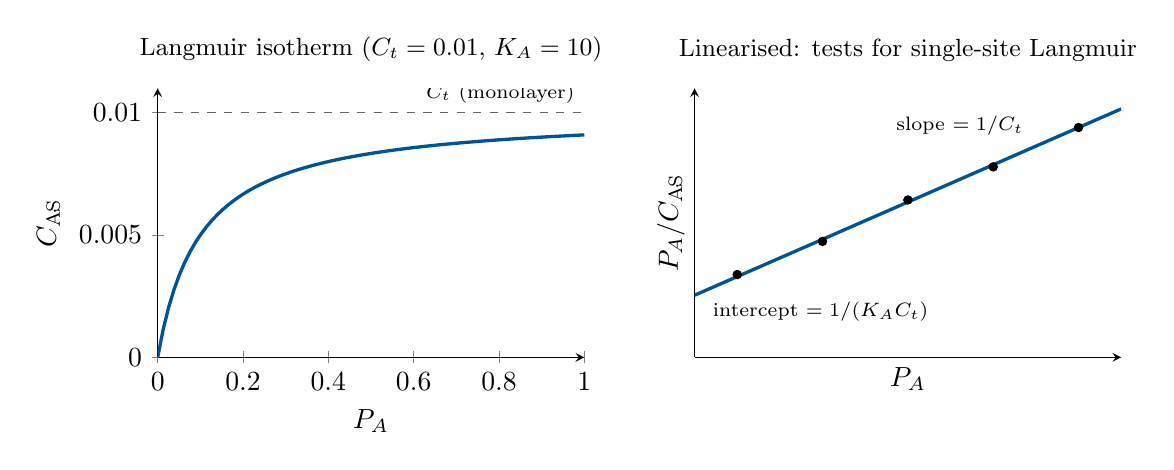
\begin{tikzpicture}
\begin{axis}[name=iso,width=7cm,height=5cm,xmin=0,xmax=1,ymin=0,ymax=0.011,axis lines=left,
  xlabel={$P_A$},ylabel={$C_{\AS{A}}$},scaled y ticks=false,yticklabel style={/pgf/number format/fixed,/pgf/number format/precision=3},
  title={\small Langmuir isotherm ($C_t=0.01$, $K_A=10$)}]
\addplot[very thick,keyblue,domain=0:1,samples=80]{0.01*10*x/(1+10*x)};
\addplot[dashed,black!60] coordinates{(0,0.01)(1,0.01)};
\node[font=\scriptsize,anchor=south east] at (axis cs:1,0.01) {$C_t$ (monolayer)};
\end{axis}
\begin{axis}[at={(iso.east)},anchor=west,xshift=1.4cm,width=7cm,height=5cm,axis lines=left,xmin=0,xmax=1,ymin=0,ymax=1.3,
  xlabel={$P_A$},ylabel={$P_A/C_{\AS{A}}$},ticks=none,title={\small Linearised: tests for single-site Langmuir}]
\addplot[very thick,keyblue,domain=0:1]{0.3+0.9*x};
\addplot[only marks,mark=*,mark size=1.5pt] coordinates{(0.1,0.40)(0.3,0.56)(0.5,0.76)(0.7,0.92)(0.9,1.11)};
\node[font=\scriptsize,anchor=west] at (axis cs:0.02,0.22) {intercept $=1/(K_AC_t)$};
\node[font=\scriptsize,anchor=west] at (axis cs:0.45,1.12) {slope $=1/C_t$};
\end{axis}
\end{tikzpicture}
\end{center}

\subsubsection*{(b) Dissociative (atomic) adsorption: \ce{A2 + 2S <=> 2A.S}}
Two vacant sites are needed, and two adsorbed atoms must recombine to desorb:
\[
r_{AD}=k_AP_{A_2}C_v^2-k_{-A}C_{\AS{A}}^2=k_A\left(P_{A_2}C_v^2-\frac{C_{\AS{A}}^2}{K_A}\right).
\]
\step{1}At equilibrium: $C_{\AS{A}}^2=K_AP_{A_2}C_v^2\Rightarrow C_{\AS{A}}=(K_AP_{A_2})^{1/2}C_v$.

\step{2}Site balance: $C_t=C_v\left[1+(K_AP_{A_2})^{1/2}\right]$.

\step{3}
\begin{keyresult}[Dissociative Langmuir isotherm]
\[
C_{\AS{A}}=\frac{(K_AP_{A_2})^{1/2}C_t}{1+(K_AP_{A_2})^{1/2}}
\qquad\Longleftrightarrow\qquad
\frac{1}{C_{\AS{A}}}=\frac{1}{C_t}+\frac{1}{C_t\sqrt{K_A}}\cdot\frac{1}{\sqrt{P_{A_2}}}
\]
\textbf{Signature: square roots of pressure.} To test, plot $1/C_{\AS{A}}$ against $1/\sqrt{P}$: a straight line means dissociative.
\end{keyresult}

\subsubsection*{(c) Several species competing for the same sites}
For \ce{A + S <=> A.S} and \ce{B + S <=> B.S}, each one at equilibrium gives $C_{\AS{i}}=K_iP_iC_v$.
The site balance $C_t=C_v+C_{\AS{A}}+C_{\AS{B}}$ gives
\[
C_v=\frac{C_t}{1+K_AP_A+K_BP_B},\qquad
C_{\AS{A}}=\frac{K_AP_AC_t}{1+K_AP_A+K_BP_B}.
\]
\textbf{General rule:} the site balance always gives $C_v=C_t\big/\left(1+\sum_i(\text{adsorbed term of }i)\right)$, where the
term is $K_iP_i$ for molecular adsorption and $\sqrt{K_iP_i}$ for dissociative adsorption.

\subsection{Surface reactions and desorption}
\fogler{4th ed.\ pp.~666--669}

\begin{center}
\small
\renewcommand{\arraystretch}{1.45}
\begin{tabular}{lll}
\toprule
Type & Step & Rate law ($K_S$ = surface equilibrium constant)\\
\midrule
Single site (L--H) & \ce{A.S <=> B.S} & $r_S=k_S\left(C_{\AS{A}}-\dfrac{C_{\AS{B}}}{K_S}\right)$\\
Dual site, adjacent vacant site & \ce{A.S + S <=> B.S + S} & $r_S=k_S\left(C_{\AS{A}}C_v-\dfrac{C_{\AS{B}}C_v}{K_S}\right)$\\
Dual site, two adsorbed species & \ce{A.S + B.S <=> C.S + D.S} & $r_S=k_S\left(C_{\AS{A}}C_{\AS{B}}-\dfrac{C_{\AS{C}}C_{\AS{D}}}{K_S}\right)$\\
Eley--Rideal (gas attacks) & \ce{A.S + B(g) <=> C.S} & $r_S=k_S\left(C_{\AS{A}}P_B-\dfrac{C_{\AS{C}}}{K_S}\right)$\\
\midrule
Desorption & \ce{C.S <=> C + S} & $r_D=k_D\left(C_{\AS{C}}-K_CP_CC_v\right)$\\
\bottomrule
\end{tabular}
\end{center}
Examples: single site, isomerisation; dual site, dehydration of alcohols; two adsorbed species, \ce{CO + O -> CO2};
the variant on two different site types is $\AS{A}+\mathrm{B\!\cdot\!S'}\rightleftharpoons\mathrm{C\!\cdot\!S'}+\AS{D}$.
For desorption, $K_C$ is the \emph{adsorption} constant of C, so a desorption step at equilibrium gives $C_{\AS{C}}=K_CP_CC_v$,
the same as adsorption.

\subsection{The rate-limiting-step method}
\fogler{4th ed.\ p.~669; 5th ed.\ Ch.~10}

At steady state the steps are in series, so $-r_A'=r_{AD}=r_S=r_D$. One step is slow (it has a small $k$ and controls
the rate). The \textbf{other steps are fast}: their $k$ is huge but their rate is finite, so their bracket must be
almost zero. They are \textbf{effectively at equilibrium}:
\[
\frac{r_{\text{fast}}}{k_{\text{fast}}}\approx0 .
\]
\begin{keyresult}[Langmuir--Hinshelwood protocol (memorise these 7 steps)]
\begin{enumerate}
\item Propose a mechanism (molecular or dissociative adsorption; single site, dual site, or Eley--Rideal).
\item Write the net rate law for every step.
\item Pick a rate-limiting step (RLS). Its rate law \textbf{is} the overall rate.
\item Set every other step at equilibrium ($r/k\approx0$) and solve for each $C_{i\cdot S}$ in terms of the $P_i$ and $C_v$.
\item Substitute these into the RLS rate law, so that only $C_v$ and the $P_i$ remain.
\item Write the total site balance and solve for $C_v$.
\item Substitute $C_v$, group the constants, and check: at equilibrium, the rate must be zero when $P_B/P_A=K_P$.
\end{enumerate}
\end{keyresult}

\begin{examtip}[Consistency check on the overall equilibrium constant]
The overall $K_P$ is the product of the step equilibrium constants, with desorption contributing $1/K_i$.
For \ce{A <=> B} via adsorb--react--desorb: $K_P=\dfrac{K_AK_S}{K_B}$. Your final rate law must contain $(P_A-P_B/K_P)$.
\end{examtip}

% ---------------------------------------------------------------------
\subsection{Example 1: Surface reaction limiting (the most common case, $>75\%$ of reactions)}
Mechanism, \ce{A <=> B}:\quad
\ce{A + S <=> A.S} (fast),\quad \underline{\ce{A.S <=> B.S}} (RLS),\quad \ce{B.S <=> B + S} (fast).

\step{1}\textbf{RLS rate law:} $-r_A'=r_S=k_S\left(C_{\AS{A}}-\dfrac{C_{\AS{B}}}{K_S}\right)$.

\step{2}\textbf{Fast steps at equilibrium:}
\[
\frac{r_{AD}}{k_A}=P_AC_v-\frac{C_{\AS{A}}}{K_A}\approx0\Rightarrow C_{\AS{A}}=K_AP_AC_v;\qquad
\frac{r_D}{k_D}=C_{\AS{B}}-K_BP_BC_v\approx0\Rightarrow C_{\AS{B}}=K_BP_BC_v.
\]
\step{3}\textbf{Substitute into the RLS:}
\[
r_S=k_SC_v\left(K_AP_A-\frac{K_B}{K_S}P_B\right)=k_SK_AC_v\left(P_A-\frac{K_B}{K_AK_S}P_B\right)=k_SK_AC_v\left(P_A-\frac{P_B}{K_P}\right),
\quad K_P=\frac{K_AK_S}{K_B}.
\]
\step{4}\textbf{Site balance:} $C_t=C_v+K_AP_AC_v+K_BP_BC_v\Rightarrow C_v=\dfrac{C_t}{1+K_AP_A+K_BP_B}$.

\step{5}\textbf{Final:}
\begin{keyresult}[Surface reaction limiting, single site]
\[
-r_A'=\frac{k\left(P_A-P_B/K_P\right)}{1+K_AP_A+K_BP_B},\qquad k=k_SK_AC_t,\quad K_P=\frac{K_AK_S}{K_B}.
\]
Initial rate (no B in the feed): $-r_{A0}'=\dfrac{kP_{A0}}{1+K_AP_{A0}}$. It is linear at low $P_{A0}$ and levels off at $k/K_A$ at high $P_{A0}$.
\end{keyresult}
\begin{mistake}[Slide notation]
The slides write $(P_A-K_eP_B)$ with $K_e=K_B/(K_AK_S)$ in Example 1, but $(P_A-P_B/K_e)$ with $K_e=K_AK_S/K_B$ in
Example 2. They are reciprocals of each other. These notes use one constant throughout: $K_P=K_AK_S/K_B$, the true
equilibrium constant $(P_B/P_A)_{\text{eq}}$, as in Fogler.
\end{mistake}

% ---------------------------------------------------------------------
\subsection{Example 2: Adsorption of A limiting}
Same mechanism, but now \underline{\ce{A + S <=> A.S}} is the RLS.

\step{1}\textbf{RLS rate law:} $-r_A'=r_{AD}=k_A\left(P_AC_v-\dfrac{C_{\AS{A}}}{K_A}\right)$.

\step{2}\textbf{Fast steps at equilibrium:}
\[
\frac{r_S}{k_S}=C_{\AS{A}}-\frac{C_{\AS{B}}}{K_S}\approx0\Rightarrow C_{\AS{A}}=\frac{C_{\AS{B}}}{K_S};\qquad
C_{\AS{B}}=K_BP_BC_v\;\Rightarrow\;C_{\AS{A}}=\frac{K_BP_B}{K_S}C_v .
\]
Note that $C_{\AS{A}}$ is set by the \emph{products}, not by $P_A$: A on the surface is in equilibrium with B.

\step{3}\textbf{Substitute:}
$r_{AD}=k_AC_v\left(P_A-\dfrac{K_B}{K_SK_A}P_B\right)=k_AC_v\left(P_A-\dfrac{P_B}{K_P}\right)$.

\step{4}\textbf{Site balance:}
\[
C_t=C_v+\frac{K_BP_B}{K_S}C_v+K_BP_BC_v=C_v\left[1+\frac{K_A}{K_P}P_B+K_BP_B\right]
\quad\left(\text{using }\frac{K_B}{K_S}=\frac{K_A}{K_P}\right).
\]
\step{5}\textbf{Final:}
\begin{keyresult}[Adsorption of A limiting]
\[
-r_A'=\frac{k_AC_t\left(P_A-P_B/K_P\right)}{1+\dfrac{K_A}{K_P}P_B+K_BP_B}.
\]
Initial rate ($P_B=0$): $-r_{A0}'=k_AC_tP_{A0}$, \textbf{linear in $P_{A0}$ with no levelling off}. There is no
$K_AP_A$ term in the denominator.
\end{keyresult}
\begin{mistake}[Slide typo]
The slide's denominator, $1+P_B(K_B+K_eK_B)$ (and $1+(K_B+K_eK_A)P_B$ in the $C_v$ line), is wrong. The correct
denominator is $1+K_BP_B\left(1+\frac{1}{K_S}\right)=1+\frac{K_A}{K_P}P_B+K_BP_B$.
\end{mistake}

% ---------------------------------------------------------------------
\subsection{Example 3 (for completeness): Desorption of B limiting}
Here \ce{A + S <=> A.S} and \ce{A.S <=> B.S} are fast, so $C_{\AS{A}}=K_AP_AC_v$ and
$C_{\AS{B}}=K_SC_{\AS{A}}=K_SK_AP_AC_v$. The RLS is
\[
r_D=k_D\left(C_{\AS{B}}-K_BP_BC_v\right)=k_DK_BC_v\left(\frac{K_SK_A}{K_B}P_A-P_B\right)=k_DK_BK_PC_v\left(P_A-\frac{P_B}{K_P}\right).
\]
Site balance: $C_t=C_v(1+K_AP_A+K_SK_AP_A)$, so
\[
-r_A'=\frac{k_DK_BK_PC_t\left(P_A-P_B/K_P\right)}{1+K_A(1+K_S)P_A}
\quad\Rightarrow\quad
-r_{A0}'=\frac{k'P_{A0}}{1+K_A(1+K_S)P_{A0}} .
\]
The initial rate also levels off at high $P_{A0}$, and no $P_B$ term appears in the denominator.

% ---------------------------------------------------------------------
\subsection{Diagnosing the RLS from initial-rate data}
Measure $-r_{A0}'$ against the feed pressure $P_{A0}$ with no products present. The shape of the curve identifies the mechanism:

\begin{center}
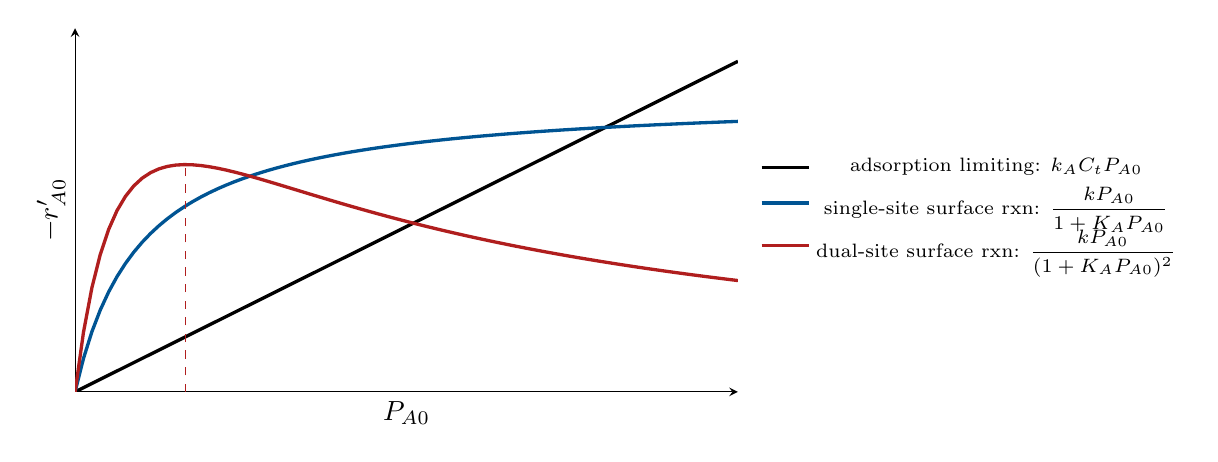
\begin{tikzpicture}
\begin{axis}[width=10cm,height=6.2cm,xmin=0,xmax=10,ymin=0,ymax=2.2,axis lines=left,
  xlabel={$P_{A0}$},ylabel={$-r_{A0}'$},ticks=none,
  legend style={font=\scriptsize,at={(1.02,0.5)},anchor=west,draw=none}]
\addplot[very thick,black,domain=0:10]{0.2*x};
\addlegendentry{adsorption limiting: $k_AC_tP_{A0}$}
\addplot[very thick,keyblue,domain=0:10,samples=80]{2.4*x/(1+1.0*x)*0.75};
\addlegendentry{single-site surface rxn: $\dfrac{kP_{A0}}{1+K_AP_{A0}}$}
\addplot[very thick,warnred,domain=0:10,samples=80]{6*x/(1+0.6*x)^2*0.55};
\addlegendentry{dual-site surface rxn: $\dfrac{kP_{A0}}{(1+K_AP_{A0})^2}$}
\addplot[dashed,warnred] coordinates{(1.667,0)(1.667,1.375)};
\node[font=\scriptsize,warnred,anchor=north] at (axis cs:1.667,0) {$1/K_A$};
\end{axis}
\end{tikzpicture}
\end{center}

\begin{center}
\renewcommand{\arraystretch}{1.3}
\begin{tabular}{lll}
\toprule
RLS & $-r_{A0}'$ & Linear plot for parameters\\
\midrule
Adsorption of A & $k_AC_tP_{A0}$ & $-r_{A0}'$ vs $P_{A0}$ (straight through the origin)\\
Single-site surface reaction & $\dfrac{kP_{A0}}{1+K_AP_{A0}}$ & $\dfrac{P_{A0}}{-r_{A0}'}=\dfrac{1}{k}+\dfrac{K_A}{k}P_{A0}$\\
Dual-site surface reaction & $\dfrac{kP_{A0}}{(1+K_AP_{A0})^2}$ & $\sqrt{\dfrac{P_{A0}}{-r_{A0}'}}=\dfrac{1}{\sqrt k}+\dfrac{K_A}{\sqrt k}P_{A0}$\\
\bottomrule
\end{tabular}
\end{center}
\textbf{Dual site, maximum:} $\dfrac{d}{dP}\left[\dfrac{kP}{(1+K_AP)^2}\right]=k\dfrac{(1+K_AP)-2K_AP}{(1+K_AP)^3}=0\Rightarrow P^*=\dfrac{1}{K_A}$
and $-r'_{\max}=\dfrac{k}{4K_A}$. Past the maximum, A covers so many sites that there are no \emph{vacant}
neighbouring sites left for the reaction.

% ---------------------------------------------------------------------
\subsection{Bimolecular L--H mechanism (Lecture 9): \ce{A + W <=> B}}
(The slides use liquid-phase concentrations $C_i$ instead of $P_i$. The algebra is identical.)
\begin{gather*}
\ce{A + S <=> A.S}\ (K_A),\qquad \ce{W + S <=> W.S}\ (K_W),\\
\ce{W.S + A.S <=> B.S + S}\ (K_S),\qquad \ce{B.S <=> B + S}\ (K_B).
\end{gather*}
\textbf{Rate laws of each step:}
\begin{align*}
r_A&=k_A\!\left(C_AC_v-\frac{C_{\AS{A}}}{K_A}\right), &
r_W&=k_W\!\left(C_WC_v-\frac{C_{\AS{W}}}{K_W}\right),\\
r_S&=k_S\!\left(C_{\AS{A}}C_{\AS{W}}-\frac{C_{\AS{B}}C_v}{K_S}\right), &
r_B&=k_B\!\left(\frac{C_{\AS{B}}}{K_B}-C_BC_v\right).
\end{align*}

\subsubsection*{Case (i): surface reaction limiting}
\step{1}Fast steps: $C_{\AS{A}}=K_AC_AC_v$, $C_{\AS{W}}=K_WC_WC_v$, $C_{\AS{B}}=K_BC_BC_v$.

\step{2}Substitute into $r_S$:
\[
r_S=k_S\left(K_AK_WC_AC_WC_v^2-\frac{K_BC_BC_v^2}{K_S}\right)=k_SK_AK_WC_v^2\left(C_AC_W-\frac{C_B}{K_P}\right),\quad K_P=\frac{K_SK_AK_W}{K_B}.
\]
\step{3}Site balance: $C_T=C_v(1+K_AC_A+K_WC_W+K_BC_B)$.

\step{4}
\begin{keyresult}[Bimolecular L--H, surface reaction limiting]
\[
-r_A'=\frac{k_SK_AK_WC_T^2\left(C_AC_W-C_B/K_P\right)}{\left(1+K_AC_A+K_WC_W+K_BC_B\right)^2}
\]
The denominator is \textbf{squared} because two sites take part in the RLS (it contains $C_v^2$).
\end{keyresult}

\subsubsection*{Case (ii): adsorption of A limiting}
\step{1}Fast steps: $C_{\AS{W}}=K_WC_WC_v$, $C_{\AS{B}}=K_BC_BC_v$, and surface-reaction equilibrium:
\[
C_{\AS{A}}C_{\AS{W}}=\frac{C_{\AS{B}}C_v}{K_S}\;\Rightarrow\;
C_{\AS{A}}=\frac{C_{\AS{B}}C_v}{K_SC_{\AS{W}}}=\frac{K_BC_BC_v}{K_SK_WC_W}=\frac{K_A}{K_P}\frac{C_B}{C_W}C_v .
\]
\step{2}RLS: $r_A=k_AC_v\left(C_A-\dfrac{C_B}{K_PC_W}\right)$.

\step{3}Site balance: $C_T=C_v\left(1+\dfrac{K_AC_B}{K_PC_W}+K_WC_W+K_BC_B\right)$.

\step{4}
\begin{keyresult}[Bimolecular, adsorption of A limiting]
\[
-r_A'=\frac{k_AC_T\left(C_A-\dfrac{C_B}{K_PC_W}\right)}{1+K_WC_W+K_BC_B+\dfrac{K_AC_B}{K_PC_W}}
\]
\end{keyresult}
\begin{mistake}[Slide typo]
On the slide, the last denominator term is printed as $C_B/(K_PC_W)$, and the $C_{\AS{A}}$ line omits $K_B$. The correct
term is $K_AC_B/(K_PC_W)$. Check: it must equal $C_{\AS{A}}/C_v$.
\end{mistake}

% ---------------------------------------------------------------------
\subsection{Eley--Rideal kinetics (one species reacts from the gas phase)}
\ce{A + S <=> A.S} (fast), \underline{\ce{A.S + B(g) <=> C.S}} (RLS), \ce{C.S <=> C + S} (fast).

\step{1}$C_{\AS{A}}=K_AP_AC_v$, \;$C_{\AS{C}}=K_CP_CC_v$.

\step{2}$r_S=k_S\left(C_{\AS{A}}P_B-\dfrac{C_{\AS{C}}}{K_S}\right)=k_SK_AC_v\left(P_AP_B-\dfrac{P_C}{K_P}\right)$, with $K_P=\dfrac{K_AK_S}{K_C}$.

\step{3}Site balance: $C_t=C_v(1+K_AP_A+K_CP_C)$. \textbf{B does not appear}, because it never occupies a site.
\begin{keyresult}[Eley--Rideal, surface reaction limiting]
\[
-r_A'=\frac{k\left(P_AP_B-P_C/K_P\right)}{1+K_AP_A+K_CP_C},\qquad k=k_SK_AC_t .
\]
Signature: B is in the numerator but not in the denominator.
\end{keyresult}

\subsection{Working backwards: from an observed rate law to a mechanism}
Experiments often report \emph{apparent orders}, e.g.\ ``first order in A, zero order in B, $-1$ order in product C''.
\begin{itemize}
\item A \textbf{negative order} in a species means it sits in the denominator and \textbf{dominates} it. Its adsorbed
form covers most sites (e.g.\ $1+K_AP_A+K_CP_C\approx K_CP_C$).
\item A \textbf{zero order} in a reactant means its pressure cancels: either it appears to the same power in the
numerator and the dominant denominator term, or its step is fast and not involved in the RLS.
\item Write the general L--H expression, then keep only the dominant denominator term to reproduce the observed orders.
\end{itemize}
\textbf{Example:} \ce{A -> C}, surface reaction limiting, product strongly adsorbed ($K_CP_C\gg1+K_AP_A$):
\[
-r_A'=\frac{kP_A}{1+K_AP_A+K_CP_C}\approx\frac{k}{K_C}\frac{P_A}{P_C}\qquad(\text{first order in A},\ -1\text{ order in C}).
\]

% ---------------------------------------------------------------------
\subsection{Designing catalytic reactors with an L--H rate law}
\fogler{4th ed.\ \S10.4}

Use the same design equations as in Lectures 1--5, written per mass of catalyst $W$:
\[
\text{PBR: } F_{A0}\frac{dX}{dW}=-r_A',\qquad
\text{CSTR / fluidised bed: } W=\frac{F_{A0}X}{(-r_A')_{\text{exit}}}.
\]
Stoichiometry for gases: $P_A=C_ART=P_{A0}\dfrac{1-X}{1+\varepsilon X}\,y\,\dfrac{T_0}{T}$, and similarly
$P_B=P_{A0}\dfrac{\Theta_B+(b/a)X}{1+\varepsilon X}\,y$, etc.

\textbf{Worked case (PBR, analytic).} $-r_A'=\dfrac{kP_A}{1+K_AP_A}$, pure A with $\varepsilon=0$ (\ce{A -> B}), isothermal, $y=1$:
\[
W=F_{A0}\int_0^X\frac{1+K_AP_{A0}(1-X)}{kP_{A0}(1-X)}\,dX
=\frac{F_{A0}}{kP_{A0}}\left[\ln\frac{1}{1-X}+K_AP_{A0}X\right].
\]
This has the same structure as the enzyme batch equation: one first-order piece plus one zero-order piece.

\begin{center}
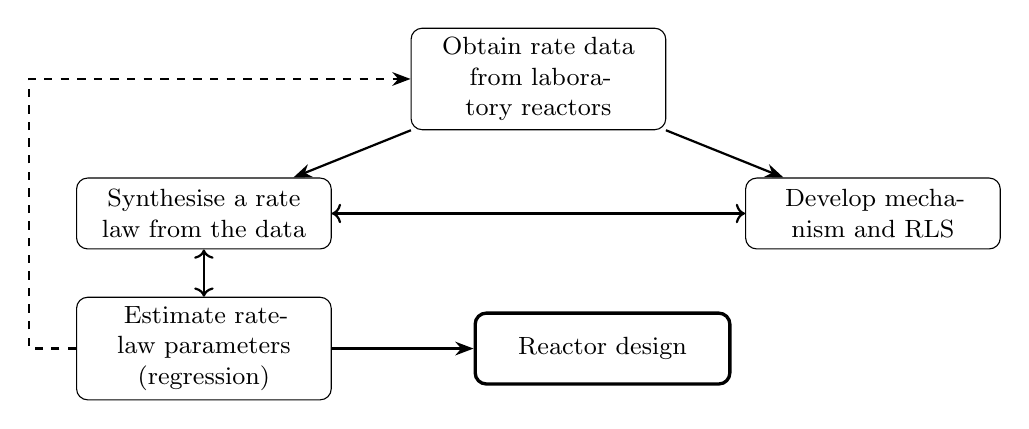
\begin{tikzpicture}[font=\small,node distance=6mm and 10mm,
  b/.style={draw,rounded corners,align=center,text width=3cm,minimum height=9mm},
  a/.style={-{Stealth},thick}]
\node[b] (d) {Obtain rate data from laboratory reactors};
\node[b,below left=of d] (s) {Synthesise a rate law from the data};
\node[b,below right=of d] (m) {Develop mechanism and RLS};
\node[b,below=of s] (e) {Estimate rate-law parameters (regression)};
\node[b,right=18mm of e,very thick] (r) {Reactor design};
\draw[a] (d)--(s); \draw[a] (d)--(m); \draw[a,<->] (s)--(m); \draw[a,<->] (s)--(e); \draw[a] (e)--(r);
\draw[a,dashed] (e.west) -- ++(-0.6,0) |- (d.west);
\end{tikzpicture}

{\small Collecting information for catalytic reactor design (Lec.~8).}
\end{center}

% =====================================================================
\section{Lecture 10: Catalytic Reactors and Catalyst Deactivation}
% =====================================================================
\fogler{4th ed.\ \S10.7, pp.~707--730}

\subsection{Industrial catalytic reactors}
\begin{center}
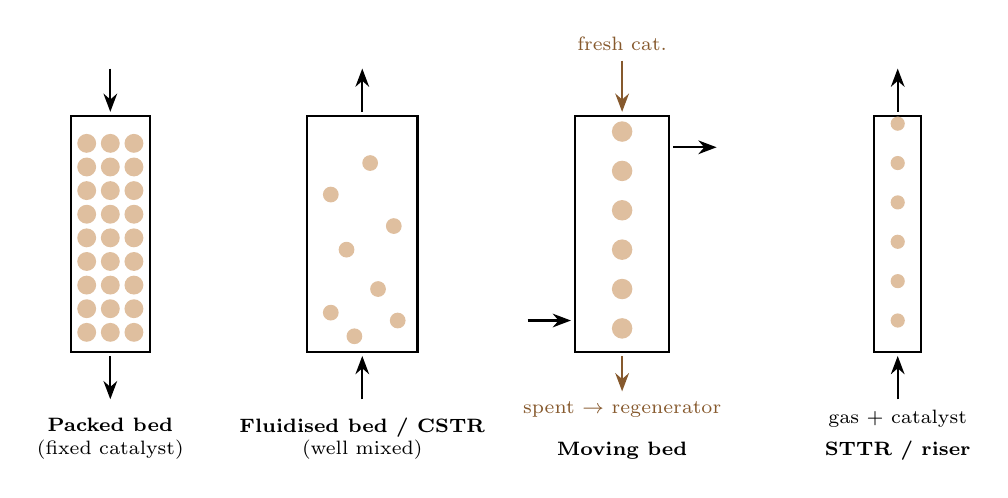
\begin{tikzpicture}[font=\scriptsize,a/.style={-{Stealth},thick}]
% PBR
\begin{scope}
\draw[thick] (0,0) rectangle (1,3);
\foreach \y in {0.25,0.55,...,2.8}{\foreach \x in {0.2,0.5,0.8}{\fill[brown!50] (\x,\y) circle(0.12);}}
\draw[a] (0.5,3.6)--(0.5,3.05); \draw[a] (0.5,-0.05)--(0.5,-0.6);
\node[align=center] at (0.5,-1.1) {\textbf{Packed bed}\\(fixed catalyst)};
\end{scope}
% fluidised CSTR
\begin{scope}[xshift=3cm]
\draw[thick] (0,0) rectangle (1.4,3);
\foreach \p in {(0.3,0.5),(0.9,0.8),(0.5,1.3),(1.1,1.6),(0.3,2.0),(0.8,2.4),(1.15,0.4),(0.6,0.2)}{\fill[brown!50] \p circle(0.1);}
\draw[a] (0.7,-0.6)--(0.7,-0.05); \draw[a] (0.7,3.05)--(0.7,3.6);
\node[align=center] at (0.7,-1.1) {\textbf{Fluidised bed / CSTR}\\(well mixed)};
\end{scope}
% moving bed
\begin{scope}[xshift=6.4cm]
\draw[thick] (0,0) rectangle (1.2,3);
\foreach \y in {0.3,0.8,...,2.8}{\fill[brown!50] (0.6,\y) circle(0.13);}
\draw[a,brown!70!black] (0.6,3.7)--(0.6,3.05) node[pos=0,above]{fresh cat.};
\draw[a,brown!70!black] (0.6,-0.05)--(0.6,-0.5) node[below]{spent $\to$ regenerator};
\draw[a] (-0.6,0.4)--(-0.05,0.4); \draw[a] (1.25,2.6)--(1.8,2.6);
\node[align=center] at (0.6,-1.25) {\textbf{Moving bed}};
\end{scope}
% STTR
\begin{scope}[xshift=10.2cm]
\draw[thick] (0,0) rectangle (0.6,3);
\foreach \y in {0.4,0.9,...,2.9}{\fill[brown!50] (0.3,\y) circle(0.09);}
\draw[a] (0.3,-0.6)--(0.3,-0.05) node[pos=0,below]{gas + catalyst};
\draw[a] (0.3,3.05)--(0.3,3.6);
\node[align=center] at (0.3,-1.25) {\textbf{STTR / riser}};
\end{scope}
\end{tikzpicture}
\end{center}

\begin{center}
\renewcommand{\arraystretch}{1.25}
\begin{tabularx}{\textwidth}{l X X}
\toprule
Reactor & Description & Typical use / when to choose it\\
\midrule
CSTR (stacked, fluidised) & Well mixed. Stacked units in series are reheated between stages for endothermic reactions (feed $\sim$1000$^\circ$F). & Water treatment, reforming. Design: $W=F_{A0}X/(-r_A')$.\\
Packed bed (PBR) & Tube filled with fixed pellets. The \textbf{highest conversion per mass of catalyst}. & Syngas, methanol, NH$_3$, Fischer--Tropsch, gas cleaning. Best when the catalyst decays \textbf{slowly}.\\
Moving bed (MBR) & Catalyst flows with the reactants, is separated, regenerated (coke burned off at $\sim$1400$^\circ$F) and recycled. & Catalytic cracking. \textbf{Moderate} decay (hours to days).\\
STTR (straight-through transport) & Gas carries the catalyst straight through; fed continuously. & Gasoline from heavy oil, F--T at Sasol. \textbf{Fast} decay (seconds), so ``decay disguise'' is eliminated.\\
\bottomrule
\end{tabularx}
\end{center}

\textbf{Catalysts and supports.} Some catalysts are the active material only; most are an active phase on a support.
\textbf{Zeolites} are crystalline aluminosilicates with molecular-size channels ($\sim$1~nm), which give shape
selectivity (e.g.\ LaY zeolite for cracking). \textbf{SBA-15} is an ordered mesoporous silica with larger pores.
Examples of active phase on support: Pt--Rh/Al$_2$O$_3$ (auto exhaust), Fe/K/Al$_2$O$_3$ (NH$_3$),
Ni/Al$_2$O$_3$ (steam reforming), Co/SiO$_2$ and Fe/K/Cu/SiO$_2$ (Fischer--Tropsch), Pt/Al$_2$O$_3$ (CO oxidation).

\subsection{Separable kinetics and catalyst activity}
\begin{keyresult}[Activity]
If the kinetics are \textbf{separable}, the rate on a used catalyst is the fresh rate times an activity:
\[
-r_A'=a(t)\times\left(-r_A'\right)_{\text{fresh}}=a(t)\,k(T)\,f(C_i),\qquad
a(t)=\frac{-r_A'(t)}{-r_A'(t=0)},\quad a(0)=1 .
\]
The decay law is $r_d=-\dfrac{da}{dt}=p(a)\,k_d(T)\,h(C_i)$, where $p(a)$ is usually $a^n$ and $h(C_i)$ depends on the
concentrations of poison or coke precursor.
If the kinetics are \textbf{non-separable}, $-r_A'=f(\text{catalyst history},\text{kinetics})$ and the two cannot be studied separately.
\end{keyresult}
Commercial reactors keep production constant as $a$ falls by \textbf{raising $T$}, which increases $k$ (see the trajectory below).

\subsection{Mechanism 1: Sintering (ageing, thermal degradation)}
\fogler{4th ed.\ p.~711}
\begin{itemize}
\item Loss of active surface area after long exposure to high temperatures: crystallites grow and agglomerate, pores
narrow or collapse, the support area is lost, and the surface recrystallises.
\item Two models of crystallite growth: \textbf{(A) atomic migration}, where atoms leave small crystallites and join large ones,
and \textbf{(B) crystallite migration}, where whole crystallites move and merge.
\item Slow, \textbf{irreversible} (or hard to reverse): sintering is \emph{prevented} rather than cured.
\end{itemize}
\begin{center}
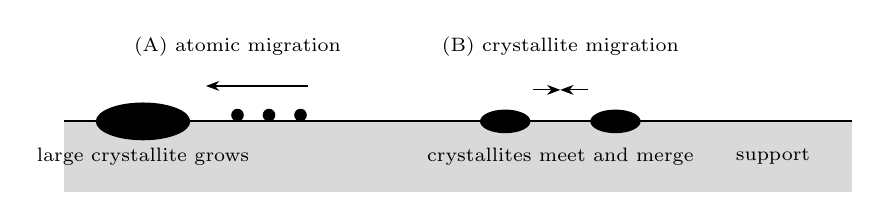
\begin{tikzpicture}[font=\scriptsize]
\fill[black!15] (0,0) rectangle (10,-0.9);
\draw[thick] (0,0)--(10,0);
\node at (9.0,-0.45) {support};
% (A) atomic migration
\fill[black] (1.0,0) ellipse (0.6 and 0.24);
\foreach \x in {2.2,2.6,3.0}{\fill[black] (\x,0.08) circle (0.08);}
\draw[-{Stealth}] (3.1,0.45)--(1.8,0.45);
\node at (2.2,0.95) {(A) atomic migration};
\node at (1.0,-0.45) {large crystallite grows};
% (B) crystallite migration
\fill[black] (5.6,0) ellipse (0.32 and 0.15);
\fill[black] (7.0,0) ellipse (0.32 and 0.15);
\draw[-{Stealth}] (5.95,0.4)--(6.3,0.4); \draw[-{Stealth}] (6.65,0.4)--(6.3,0.4);
\node at (6.3,0.95) {(B) crystallite migration};
\node at (6.3,-0.45) {crystallites meet and merge};
\end{tikzpicture}
\end{center}

\textbf{Sintering is typically second order in activity.} Derivation:
\[
r_d=-\frac{da}{dt}=k_da^2
\;\Rightarrow\;
\int_1^{a}\frac{da}{a^2}=-k_d\int_0^t dt
\;\Rightarrow\;
\left[-\frac{1}{a}\right]_1^{a}=-k_dt
\;\Rightarrow\;
\frac{1}{a}-1=k_dt .
\]
\begin{keyresult}[Sintering (second-order decay)]
\[
a(t)=\frac{1}{1+k_dt},\qquad k_d(T)=k_d(T_0)\exp\!\left[\frac{E_d}{R}\left(\frac{1}{T_0}-\frac{1}{T}\right)\right].
\]
Test the data by plotting $1/a$ against $t$: a straight line with slope $k_d$ and intercept 1.
\end{keyresult}

\begin{center}
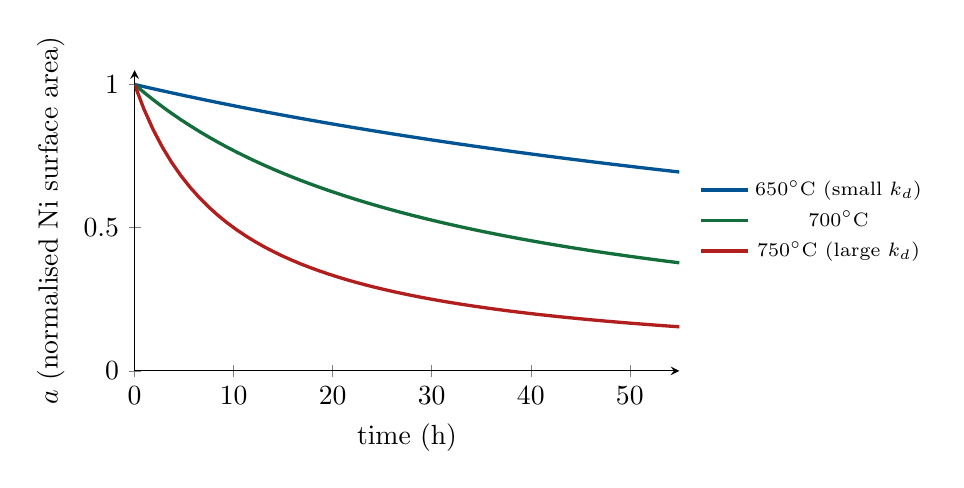
\begin{tikzpicture}
\begin{axis}[width=8.5cm,height=5.4cm,xmin=0,xmax=55,ymin=0,ymax=1.05,axis lines=left,
  xlabel={time (h)},ylabel={$a$ (normalised Ni surface area)},
  legend style={font=\scriptsize,at={(1.02,0.5)},anchor=west,draw=none}]
\addplot[very thick,keyblue,domain=0:55,samples=60]{1/(1+0.008*x)};\addlegendentry{650$^\circ$C (small $k_d$)}
\addplot[very thick,tipgreen,domain=0:55,samples=60]{1/(1+0.03*x)};\addlegendentry{700$^\circ$C}
\addplot[very thick,warnred,domain=0:55,samples=60]{1/(1+0.1*x)};\addlegendentry{750$^\circ$C (large $k_d$)}
\end{axis}
\end{tikzpicture}

{\small Shape of the 13.5\% Ni/SiO$_2$ sintering data (J.~Catal.\ 81 (1983) 131): higher $T$ gives faster loss of area.}
\end{center}

\textbf{What changes the sintering rate:} it grows exponentially with $T$ ($E_d\approx30$--150~kJ/mol). It depends on the
atmosphere (for supported Pt the rate decreases in the order NO $>$ O$_2$ $>$ H$_2$ $>$ N$_2$), on the metal (stability in H$_2$: Ru $>$ Ir $\approx$ Rh $>$ Pt),
on the support (Al$_2$O$_3$ $>$ SiO$_2$ $>$ carbon in stability), on promoters (Ba, Ca, Sr oxides trap atoms and slow sintering;
Pb, Bi, Cl, F, S speed it up), and on pores (porous supports sinter more slowly).

\subsection{Mechanism 2: Poisoning}
\begin{itemize}
\item \textbf{Strong (irreversible) chemisorption} of a reactant, product or \textbf{impurity} on active sites.
Sulfur is the classic poison in petrochemical processing.
\item ``Poison'' has an operational meaning: O$_2$ is a \emph{reactant} for ethylene oxidation on Ag, but a \emph{poison} for
ethylene hydrogenation on Ni. Poisons also change the electronic and geometric structure of the surface.
\item Usually \textbf{irreversible}, so poisons are removed \emph{before} the reactor, e.g.\ hydrodesulfurisation or a
ZnO guard bed upstream of a Ni steam reformer.
\end{itemize}
\begin{center}
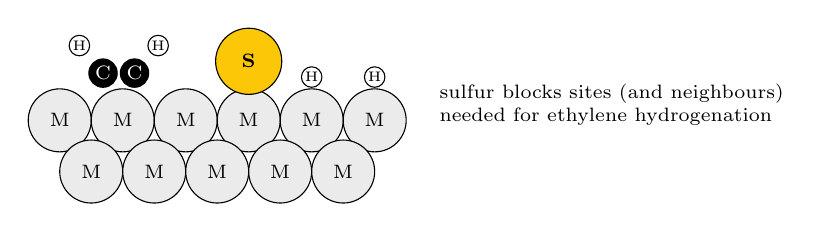
\begin{tikzpicture}[font=\scriptsize]
\foreach \i in {0,...,5}{\draw[fill=black!8] (\i*0.8,0) circle(0.4); \node at (\i*0.8,0){M};}
\foreach \i in {0,...,4}{\draw[fill=black!8] (\i*0.8+0.4,-0.65) circle(0.4); \node at (\i*0.8+0.4,-0.65){M};}
\draw[fill=yellow!60!orange] (2.4,0.75) circle(0.42); \node at (2.4,0.75) {\textbf{S}};
\draw[fill=black] (0.55,0.6) circle(0.18); \draw[fill=black] (0.95,0.6) circle(0.18);
\node[text=white] at (0.55,0.6){C}; \node[text=white] at (0.95,0.6){C};
\foreach \p in {(0.25,0.95),(1.25,0.95)}{\draw[fill=white] \p circle(0.13); \node at \p {\tiny H};}
\foreach \p in {(3.2,0.55),(4.0,0.55)}{\draw[fill=white] \p circle(0.13); \node at \p {\tiny H};}
\node[anchor=west,align=left] at (4.7,0.2) {sulfur blocks sites (and neighbours)\\needed for ethylene hydrogenation};
\end{tikzpicture}
\end{center}

\textbf{Poisoning kinetics.} Mechanism: \ce{A + S <=> A.S}, \ce{A.S <=> B.S}, \ce{B.S <=> B + S}, plus the poison
\ce{P + S -> P.S} (irreversible). Then
\[
-r_A'=a(t)\left[\frac{kP_A}{1+K_AP_A+K_BP_B}\right],\qquad
r_d=-\frac{da}{dt}=k_dP_P^{\,n}a^q=k_d'a^q,
\]
where $k_d'=k_dP_P^n$ is constant when the impurity pressure $P_P$ is constant.
\textbf{Integrate} (for $q\neq1$):
\[
\int_1^a a^{-q}\,da=-k_d'\int_0^tdt\;\Rightarrow\;\frac{a^{1-q}-1}{1-q}=-k_d't\;\Rightarrow\;
\boxed{\,a=\left[1-(1-q)k_d't\right]^{1/(1-q)}\,}
\]
For $q=1$: $a=e^{-k_d't}$. For $q=2$: $a=1/(1+k_d't)$, the same form as sintering. For $q<1$ the activity reaches
zero in a finite time, $t=1/[(1-q)k_d']$.

\textbf{Poisons for important catalysts (condensed from the slide tables):}
\begin{center}
\small
\renewcommand{\arraystretch}{1.15}
\begin{tabular}{lll}
\toprule
Catalyst & Reaction & Poisons\\
\midrule
Silica--alumina, zeolites & Cracking & organic bases, heavy metals\\
Ni, Pt, Pd & (De)hydrogenation & S, P, As, Zn, Hg, halides, Pb, NH$_3$, C$_2$H$_2$\\
Ni & Steam reforming & H$_2$S, As\\
Fe, Ru & NH$_3$ synthesis & O$_2$, H$_2$O, CO, S, C$_2$H$_2$\\
Co, Fe & Fischer--Tropsch & H$_2$S, COS, As, NH$_3$, metal carbonyls\\
Ag & Ethylene oxidation & C$_2$H$_2$\\
Pt, Pd & CO / HC oxidation & Pb, P, Zn, SO$_2$, Fe\\
\bottomrule
\end{tabular}
\end{center}
By chemical type: Group VA/VIA (N, P, As, S, Se\ldots) and Group VIIA (halogens) act through s- and p-orbitals;
toxic heavy metals (As, Pb, Hg, Zn, Cu\ldots) occupy d-orbitals and may form alloys; molecules with multiple bonds
(CO, NO, HCN, benzene, acetylene) chemisorb strongly through multiple bonds and back-bonding.

\subsection{Mechanism 3: Fouling and coking}
\begin{itemize}
\item Carbonaceous deposits (coke) build up on the surface. They have two effects: \textbf{site coverage} (they block active sites) and
\textbf{pore blockage} (they create diffusion resistance, and can encapsulate crystallites).
\item Coking is not well understood mechanistically. Pore-blocking models are probabilistic: the probability that a
site is accessible depends on the pore-size distribution.
\item \textbf{Reversible}: coke can be burned off (regeneration). This is why moving beds and FCC risers have a regenerator.
The burn-off is strongly exothermic, and the heat is recovered (it drives the endothermic cracking and makes steam).
Coke formation can also be reduced by co-feeding H$_2$ or steam (which gasify carbon) or by lowering $T$.
\end{itemize}
\begin{keyresult}[Coking]
Coke on the surface follows an empirical law, $C_c=At^n$ ($A$ and $n$ depend on the feed). The activity is then one of
\[
a=\frac{1}{1+C_c^{\,p}}=\frac{1}{1+A^pt^{np}},\qquad
a=e^{-\alpha_1C_c},\qquad
a=\frac{1}{1+\alpha_2C_c}.
\]
\end{keyresult}
Chemistry: CO dissociates to atomic C$_\alpha$, which can be hydrogenated (CH$_4$), dissolve in Ni, form Ni$_3$C, or
polymerise to less reactive C$_\beta$ and then to graphitic C$_c$ (coke). Each path has its own activation energy, so
the dominant path depends on $T$.

\textbf{Solid-state reactions that create inactive phases:} \ce{Rh2O3 + Al2O3 -> RhAl2O4} (auto catalysts),
\ce{Fe -> FeO} (NH$_3$ catalyst with $>$50~ppm O$_2$ or H$_2$O/H$_2>0.16$),
\ce{SO3 + Al2O3 -> Al2(SO4)3} (blocks pores), \ce{Ni + Al2O3 -> NiAl2O4} (steam reforming),
\ce{Co + SiO2 -> CoO.SiO2} (F--T), and H$_2$O-induced dealumination of zeolites.

\subsection{Comparing the three mechanisms (conceptual exam questions)}
\begin{center}
\small
\renewcommand{\arraystretch}{1.3}
\begin{tabular}{p{2.3cm} p{4.1cm} p{2.0cm} p{2.1cm} p{4.0cm}}
\toprule
Mechanism & What happens & Reversible? & Typical $a(t)$ & Prevention / cure\\
\midrule
Sintering & crystallites grow, pores collapse, active area lost (high $T$) & no & $\dfrac{1}{1+k_dt}$ & lower $T$; stable support; trapping promoters (BaO, CaO, SrO)\\
Poisoning & strong chemisorption of an impurity, reactant or product on sites & usually no & $[1-(1-q)k_d't]^{\frac{1}{1-q}}$ & remove the poison upstream (guard bed, desulfurisation)\\
Fouling / coking & carbon covers sites and blocks pores & yes (burn-off) & $\dfrac{1}{1+A^pt^{np}}$ & regenerate (moving bed, riser); add H$_2$/steam\\
\bottomrule
\end{tabular}
\end{center}
\textbf{Reactor choice follows the decay time scale:} years, packed bed; hours to days, moving bed with a regenerator;
seconds, STTR or riser (catalyst and feed travel together, so there is no ``decay disguise'').

\subsection{Summary of decay laws}
\begin{center}
\renewcommand{\arraystretch}{1.45}
\begin{tabular}{llll}
\toprule
Decay order & $-da/dt$ & Integrated $a(t)$ & Typical cause\\
\midrule
Zero & $k_d$ & $1-k_dt$ & poisoning ($q=0$)\\
First & $k_da$ & $e^{-k_dt}$ & poisoning, some sintering\\
Second & $k_da^2$ & $\dfrac{1}{1+k_dt}$ & \textbf{sintering}\\
Order $q$ & $k_d'a^q$ & $\left[1-(1-q)k_d't\right]^{1/(1-q)}$ & poisoning with a constant impurity\\
Coking & -- & $\dfrac{1}{1+A^pt^{np}}$ & coke $C_c=At^n$\\
\bottomrule
\end{tabular}
\end{center}

\subsection{Using $a(t)$ in reactor problems (exam-style applications)}
\textbf{(1) Conversion over time (slow decay).} The catalyst decays much more slowly than the gas residence time, so at each
moment the reactor is at steady state with $k\to a(t)k$. For a first-order reaction with $\varepsilon=0$ and no $\Delta P$:
\[
\text{PBR: } X(t)=1-\exp\!\left[-\frac{a(t)\,k'W}{v_0}\right],\qquad
\text{CSTR (fluidised, uniform $a$): } X(t)=\frac{a(t)\,k'W/v_0}{1+a(t)\,k'W/v_0}.
\]
\textbf{(2) Keeping conversion constant by lowering the feed.} Conversion depends on the group $a\,k'W/F_{A0}$ (or $a\,k'W/v_0$),
so to keep $X$ fixed you set $F_{A0}(t)=a(t)\,F_{A0}(0)$.

\textbf{(3) Temperature--time trajectory (raise $T$ to keep the rate constant).} Constant rate at constant composition
needs $a(t)\,k(T)=k(T_0)$:
\[
a(t)\exp\!\left[\frac{E}{R}\left(\frac{1}{T_0}-\frac{1}{T}\right)\right]=1
\;\Rightarrow\;
\frac{1}{T}=\frac{1}{T_0}+\frac{R}{E}\ln a(t).
\]
With sintering, $a=1/(1+k_dt)$, this gives $\dfrac1T=\dfrac{1}{T_0}-\dfrac{R}{E}\ln(1+k_dt)$ (ignoring the $T$-dependence of $k_d$).
The real plant limit is reached when $T$ hits a material or selectivity limit; then the catalyst is regenerated or replaced.
\begin{mistake}
Raising $T$ also speeds up \emph{sintering} ($k_d$ increases), so this strategy shortens catalyst life.
If an exam problem gives $E_d$, you must include $k_d(T)$.
\end{mistake}

\subsection{Course map}
\begin{center}
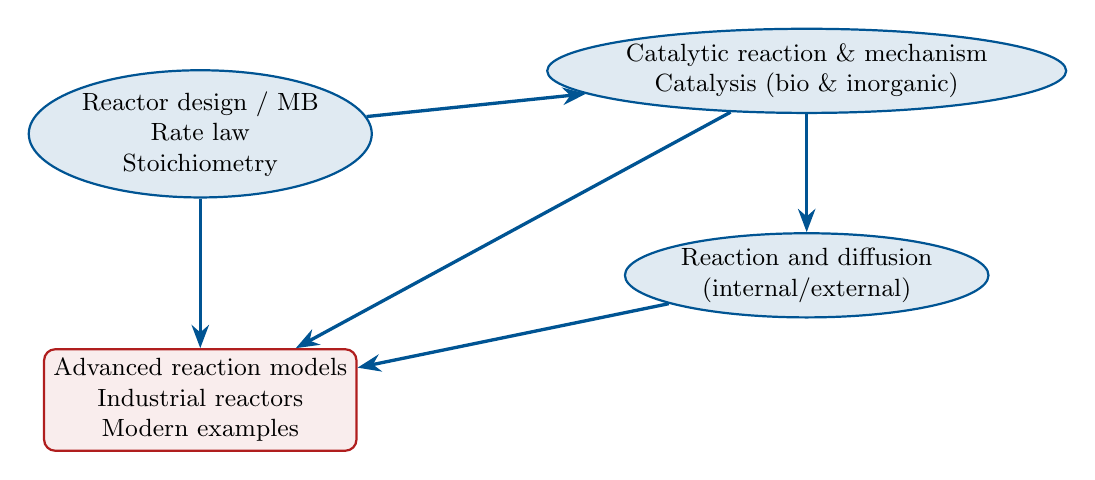
\begin{tikzpicture}[font=\small,
  e/.style={ellipse,draw=keyblue,fill=keyblue!12,thick,align=center,inner sep=1pt},
  a/.style={-{Stealth},very thick,keyblue}]
\node[e] (r) {Reactor design / MB\\Rate law\\Stoichiometry};
\node[e,right=2.2cm of r,yshift=0.8cm] (c) {Catalytic reaction \& mechanism\\Catalysis (bio \& inorganic)};
\node[e,below=1.5cm of c] (d) {Reaction and diffusion\\(internal/external)};
\node[draw=warnred,fill=warnred!8,thick,rounded corners,align=center,below=1.9cm of r] (adv) {Advanced reaction models\\Industrial reactors\\Modern examples};
\draw[a] (r)--(c); \draw[a] (c)--(d); \draw[a] (r)--(adv); \draw[a] (d)--(adv); \draw[a] (c)--(adv);
\end{tikzpicture}

{\small Lectures 1--5: left bubble. Lectures 6--10: top bubble. Next: diffusion.}
\end{center}

% =====================================================================
\newpage
\section{Formula Summary (Lectures 6--10)}
% =====================================================================
\small
\begin{multicols}{2}
\textbf{PSSH.} $r_{A^*}=\sum_ir_{iA^*}=0$. Convert each step's rate to the intermediate using
$\frac{r_A}{-a}=\frac{r_B}{-b}=\frac{r_C}{c}$ (factors of 2 and $\tfrac12$!).

\textbf{Lindemann.} $-r_A=\dfrac{k_1k_3C_A^2}{k_3+k_2C_A}$: 2nd order at low $C_A$, 1st order at high $C_A$.

\textbf{Inert collider.} $-r_A=\dfrac{k_1k_3C_AC_I}{k_3+k_2C_I}\to\dfrac{k_1k_3}{k_2}C_A$.

\textbf{NO oxidation.} $r_{\mathrm{NO_2}}=\dfrac{k_1k_3}{k_2}C_{\mathrm{NO}}^2C_{\mathrm{O_2}}$, \;$E_{\text{app}}=E_1+E_3-E_2$ (can be $<0$).

\textbf{Chain (H$_2$/Br$_2$).} Initiation = termination: $2k_1C_{\mathrm{Br_2}}=k_5C_{\mathrm{Br}\bullet}^2$.
\[
r_{\mathrm{HBr}}=\frac{2k_2\sqrt{2k_1/k_5}\,C_{\mathrm{H_2}}C_{\mathrm{Br_2}}^{3/2}}{C_{\mathrm{Br_2}}+(k_4/k_3)C_{\mathrm{HBr}}}
\]

\textbf{Michaelis--Menten.} $-r_S=\dfrac{V_{\max}C_S}{K_M+C_S}$, \;$V_{\max}=k_{\text{cat}}C_{E,t}$,
\;$K_M=\dfrac{k_2+k_3}{k_1}=S_{1/2}$.

\textbf{Lineweaver--Burk.} $\dfrac{1}{-r_S}=\dfrac{1}{V_{\max}}+\dfrac{K_M}{V_{\max}}\dfrac{1}{C_S}$.

\textbf{Hanes--Woolf.} $\dfrac{C_S}{-r_S}=\dfrac{K_M}{V_{\max}}+\dfrac{C_S}{V_{\max}}$.

\textbf{Eadie--Hofstee.} $-r_S=V_{\max}-K_M\dfrac{-r_S}{C_S}$.

\textbf{Batch enzyme.} $t=\dfrac{K_M}{V_{\max}}\ln\dfrac{1}{1-X}+\dfrac{C_{S0}X}{V_{\max}}$.

\textbf{Inhibition} ($\phi=1+C_I/K_I$):
\begin{itemize}[leftmargin=*]
\item competitive: $\dfrac{V_{\max}C_S}{C_S+K_M\phi}$ (slope $\times\phi$)
\item uncompetitive: $\dfrac{V_{\max}C_S}{K_M+C_S\phi}$ (intercept $\times\phi$)
\item noncompetitive: $\dfrac{V_{\max}C_S}{(K_M+C_S)\phi}$ (both $\times\phi$)
\end{itemize}
\vfill
\columnbreak

\textbf{Langmuir isotherms.}
\[
C_{\AS{A}}=\frac{K_AP_AC_t}{1+K_AP_A},\qquad C_{\AS{A}}=\frac{\sqrt{K_AP_A}\,C_t}{1+\sqrt{K_AP_A}}
\]
\textbf{Fast step at equilibrium.} $C_{\AS{i}}=K_iP_iC_v$ (or $\sqrt{K_iP_i}C_v$ if dissociative).

\textbf{Site balance.} $C_t=C_v+\sum_iC_{\AS{i}}$.

\textbf{\ce{A <=> B} with $K_P=K_AK_S/K_B$:}
\begin{itemize}[leftmargin=*]
\item surface rxn RLS: $\dfrac{k(P_A-P_B/K_P)}{1+K_AP_A+K_BP_B}$
\item adsorption RLS: $\dfrac{k_AC_t(P_A-P_B/K_P)}{1+\frac{K_A}{K_P}P_B+K_BP_B}$
\item desorption RLS: $\dfrac{k(P_A-P_B/K_P)}{1+K_A(1+K_S)P_A}$
\end{itemize}

\textbf{Dual site.} $\dfrac{k(\ldots)}{(1+\sum K_iP_i)^2}$; the initial rate has its maximum at $P_{A0}=1/K_A$.

\textbf{Eley--Rideal.} $\dfrac{k(P_AP_B-P_C/K_P)}{1+K_AP_A+K_CP_C}$ (B not in the denominator).

\textbf{Catalytic design.} PBR $F_{A0}\frac{dX}{dW}=-r_A'$; CSTR $W=\frac{F_{A0}X}{-r_A'}$;
$P_A=P_{A0}\frac{(1-X)}{1+\varepsilon X}y\frac{T_0}{T}$.

\textbf{Deactivation.} $-r_A'=a(t)(-r_A')_{\text{fresh}}$; $-\frac{da}{dt}=k_da^n$.
\begin{itemize}[leftmargin=*]
\item sintering: $a=\dfrac{1}{1+k_dt}$
\item poisoning: $a=[1-(1-q)k_d't]^{1/(1-q)}$; $q=1$: $e^{-k_d't}$
\item coking: $C_c=At^n$, $a=\dfrac{1}{1+A^pt^{np}}$
\item $T$ trajectory: $\frac1T=\frac1{T_0}+\frac{R}{E}\ln a(t)$
\end{itemize}

\textbf{Arrhenius.} $k(T)=k(T_0)\exp\!\left[\frac{E}{R}\left(\frac{1}{T_0}-\frac1T\right)\right]$;
$R=8.314$~J/(mol\,K)$=1.987$~cal/(mol\,K).
\end{multicols}

\end{document}
